\documentclass[utf8]{frontiersSCNS} % for Science, Engineering and Humanities and Social Sciences articles
\usepackage{gensymb}
\usepackage{url,hyperref,lineno,microtype,subcaption}
\usepackage[onehalfspacing]{setspace}

\usepackage{tabularx}
%\renewcommand{\arraystretch}{1.5}
%\usepackage{rotating}
\linenumbers
\DeclareUnicodeCharacter{2212}{}
\DeclareUnicodeCharacter{0301}{}
\usepackage{wasysym} % provides \DH, \dh, \Thorn, \thorn
% Leave a blank\usepackage{amsmath}
%\DeclareMathOperator{\sign}{sign} line between paragraphs instead of using \\


\def\keyFont{\fontsize{8}{11}\helveticabold }
\def\firstAuthorLast{Balasubramanian {et~al.}} %use et al only if is more than 1 author
\def\Authors{Suryanarayanan Balasubramanian\,$^{1,*}$, Martin Hoelzle\,$^{1}$, Michael Lehning\,$^{2}$, Sonam Wangchuk \,$^{3}$, Johannes Oerlemans\,$^{4}$ and Felix Keller\,$^{5}$}
\def\Address{$^{1}$University of Fribourg, Fribourg, Switzerland\\
$^{2}$WSL Institute for Snow and Avalanche Research, Davos, Switzerland\\
$^{3}$Himalayan Institute of Alternatives Ladakh, Leh, India\\
$^{4}$Institute for Marine and Atmospheric Research, Utrecht University, Utrecht, The Netherlands\\
$^{5}$Academia Engiadina, Samedan, Switzerland}
\def\corrAuthor{Suryanarayanan Balasubramanian}

\def\corrEmail{suryanarayanan.balasubramanian@unifr.ch}



\begin{document}
\onecolumn
\firstpage{1}

\title[Artificial Ice Reservoirs]{Mass and energy balance calculations for an artificial ice reservoir (Icestupa)}

\author[\firstAuthorLast ]{\Authors}
\address{}
\correspondance{}

\extraAuth{}

\maketitle


\begin{abstract}

Artificial Ice Reservoirs (AIRs) have been successful in storing water during winter and releasing the water during
spring and summer. This has made them a reliable fresh water resource for irrigation in dry environments. Several AIRs
have been built but studies of their water storage capacity and efficiency are scarce. This study attempts to model a
cone-shaped AIR popularly called Icestupa. Important processes involved in the development and temporal evolution of
an Icestupa are calculated by a physically-based model using equations governing the heat transfer, vapour diffusion
and transport of water that undergoes phase changes.  These processes were quantified using meteorological data in
conjunction with fountain spray information (mass input of an Icestupa) to estimate the quantity of frozen, melted,
evaporated and runoff water at a location called 'Eispalast' in Fribourg, Switzerland. At this measurement site, an
Icestupa was built for model validation purposes. The model was further tested by performing sensitivity and
uncertainty study showing that the most sensitive parameters are the ice emissivity and the temperature threshold used
to determine precipitation phase. Model calculations estimate that the Eispalast Icestupa stored about 8\% of the
total water sprayed as ice. In addition, we found that reducing nozzle diameter of the fountain from 5 $mm$ to 3 $mm$
increases the storage efficiency up to 93\% without compromising on the storage duration.

\tiny
 \keyFont{ \section{Keywords:} icestupa, mass balance, water storage, climate change adaptation, geoengineering } %All article types: you may provide up to 8 keywords; at least 5 are mandatory.
\end{abstract}

\section{Introduction}

Seasonal snow cover, glaciers and permafrost are expected to change their water storage capacity due to climate change
with major consequences for downriver water supply \citep{Immerzeel_2020}. The challenges brought about by these
changes are especially important for dry mountain environments such as in Central Asia or the Andes, which directly
rely on the seasonal meltwater for their farming and drinking needs \citep{HoelzleBarandun_2019, Apel_2018,
Buytaert_2017, Chen_2016, UNGERSHAYESTEH_2013}. Some villages in Ladakh, India have already been forced to relocate
due to glacial retreat and the corresponding loss of their main fresh water resources \citep{zanskar}. 

\begin{figure} \begin{center} 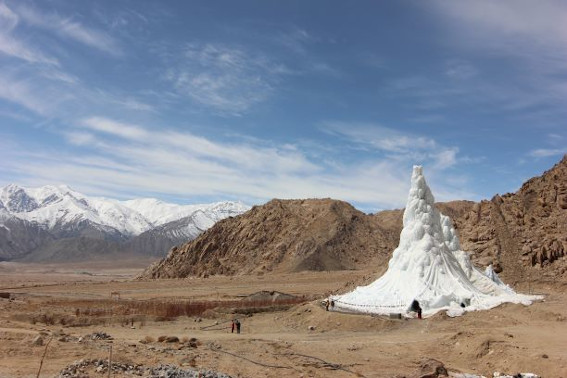
\includegraphics[width=10 cm]{Figures/Figure_1.jpg}
\end{center} \caption{Icestupa in Ladakh, India on March 2017 was 24 $m$ tall and contained around 3700 $m^3$ 
of water. Picture Credits: Lobzang Dadul} \label{fig:cone} \end{figure}

AIRs have been considered to be a feasible way to adapt to these changes \citep{IPCC_2019,
10.1659/MRD-JOURNAL-D-18-00072.1}. An artificial ice reservoir is a human-made ice structure typically constructed
during the cold winter months and designed to slowly release freshwater during the warm and dry spring and summer
months. The main purpose of AIRs is irrigation. Therefore, AIRs are designed to store water in the form of ice as long
into the summer as possible. The energy required to construct an AIR is usually derived from the gravitational head of
the source water body. Some are constructed horizontally by freezing water using a series of checkdams and others are
built vertically by spraying water through fountain systems \citep{Nusser_2018}. The latter are colloquially referred
to as Icestupas and are the subject of this study.

A typical Icestupa just requires a pipeline attached to a vertically mounted metal pipe with a fountain nozzle for
construction. Water source is usually a high altitude lake or glacial stream. Due to the altitude difference between
the pipeline input and fountain output, water ejects from the fountain nozzle as droplets that eventually lose their
latent heat to the atmosphere and accumulate as ice around the metal pipe. The fountain nozzle is raised through
addition of further pipes as and when significant ice accumulates. Typically, a dome of branches is constructed around
the metal pipe so that such pipe extensions can be done from within this dome. During the winter, the fountain is
manually activated between sunset and sunrise. Threads, tree branches and fishing nets are used to guide and accelerate
the ice formation.

Since their invention in 2013 \citep{campaign}, Icestupas have gained widespread publicity in the region of Ladakh,
Northern India since they require very little infrastructure, skills and energy to be constructed in comparison to
other water storage technologies. Compared to other AIR geometries, Icestupas (Fig.  \ref{fig:cone}) can be built at
lower altitudes and last much longer into the summer than other types of ice structures \citep{campaign}. However, to
date, no reliable estimates exist about the amount of sprayed water that is necessary to create them and the meltwater
they provide \citep{Nusser_2018}. Rough estimates of Icestupa meltwater in Ladakh suggest that the water loss during
the construction process is considerable (see Appendix \ref{section:ladakhloss}). A complete set of measurements of the
water storage and energy balance are required to understand the cause of the water losses better and increase the
construction efficiency.
 
In this paper, we aim to develop a physically-based model of a vertical AIR (or Icestupa) that can quantify their
storage efficiency using existing weather and water usage information. Mass and energy balance equations were used to
estimate the quantity of water frozen, melted, evaporated and runoff. Sensitivity and uncertainty analysis were
performed to identify the most critical parameters and the variance caused by them. For validation, we created an
Icestupa at an accessible site (called Eispalast) near Schwarzsee in the Canton of Fribourg, Switzerland, allowing easy
maintenance and control of the measurements. Due to the low altitude of the site with relatively high winter
temperatures, only a small Icestupa could be established during winter 2018/19 for providing us with model validation
data. Our model and validation experiments provide first steps towards evaluating the effectiveness of a vertical AIR
for irrigation and finally we outline some preliminary guidelines for consideration when a construction of an Icestupa
for water storage is envisaged. 

\section{Study Site}
The Eispalast (EP) site in the Schwarzsee region lies at 967 $m$ a.s.l.. In the winter (Oct-Apr), mean daily maximum
and minimum air temperatures vary between 14 to -4 $\degree C$. Clear skies are rare, averaging around 7 days, and
precipitation amounts average 155 mm per month during winter \citep{eispalast}. The site was situated adjacent to a
stream resulting in high humidity values across the study period. Within the Eispalast site, 1.8\,$m$ in radius
enclosure was constructed for the experiment. An automatic weather station (AWS) was set in place adjacent to the
wooden boundary as shown in Fig. \ref{fig:site}. The fountain used for spraying water had a nozzle diameter of 5\,$mm$
and a height of 1.35\,$m$, and was placed in the centre of the wooden enclosure. The water was transferred from a
spring water source at 1267 $m$ a.s.l. by pipeline and flowed via a flowmeter and an air escape valve to the nozzle,
where it was sprinkled with a spray radius of around 1.7\,$m$. The air escape valve was installed to avoid errors in
the flow measurements due to air bubbles. In addition, a webcam guaranteed a continuous survey of the site during the
construction of the Icestupa. 

\begin{figure}[htb] \centering \begin{tabular}{@{}cc@{}} 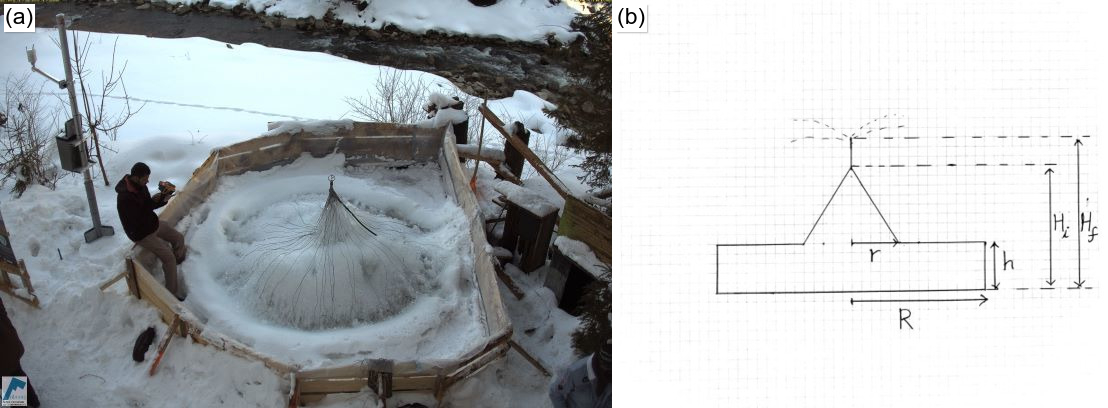
\includegraphics[width=15cm]{./Figures/Figure_2.jpg} &
\end{tabular} \caption{(a) The ice structure during the first validation measurement as seen on the webcam image of
  $14^{th}$ Feb. (b) The corresponding cross section of the EP ice structure with the field estimates of $r, R,
  h, H_i, H_f$ used to determine the Icestupa volume is shown on the right.} \label{fig:site} \end{figure}

\subsection{Construction} 
From $30^{th}$ January to $18^{th}$ March 2019 the Icestupa was constructed through the fountain spray, which was
manually switched on if measured air temperature was below -5 $\degree C$ after sunset and was switched off as soon as
the ice was exposed to daylight or temperatures were above 0 $\degree C$. The water spray of the fountain was initially
adjusted so that most of the water droplets land within the wooden boundary zone. The ice formation was guided by
adding a metal framework at the ice structure base after the first night of operation.  Several cotton threads were
tied between the ice structure base and fountain pole for accelerating and further guiding the ice formation process. 

\subsection{Measurements and Data}
The EP AWS was located at 967 $m$ a.s.l. It was in operation from $30^{th}$  January to $18^{th}$ March 2019.
Measurements comprise air temperature, relative humidity, water flow rate, wind speed and direction. All these
measurements were stored at a 5 minute sample rate. The water flow rate or discharge was measured via an ultrasonic
sensor attached to the fountain supply pipeline. Precipitation data was derived from the Plaffeien AWS
\citep{meteoswiss} located 8.8 km away from the measurement site at an altitude of 1042 $m$ a.s.l.  

ERA5 reanalysis dataset \citep{era5} correlates much better to lower elevation sites in Switzerland
\citep{Scherrer_2020}. Moreover, all the EP meteorological parameters except precipitation correlated better with ERA5
dataset compared to the nearby Plaffein AWS. Namely, the $2\,m$ temperature parameter correlated ($r^2 =0.9 $) with air
temperature, surface pressure parameter correlated ($r^2 = 1$) with air pressure and 10m wind speed parameter (derived
from horizontal and vertical components) correlated ($r^2 =0.6 $) with wind speed.  Direct and diffuse shortwave
radiation were also derived from ERA5 surface solar radiation downwards and total sky direct solar radiation parameter.
The hourly ERA5 data and the 10 minute Plaffeien AWS data were linearly interpolated to the 5 minute data frequency of
the EP AWS. 

\begin{figure} \centering 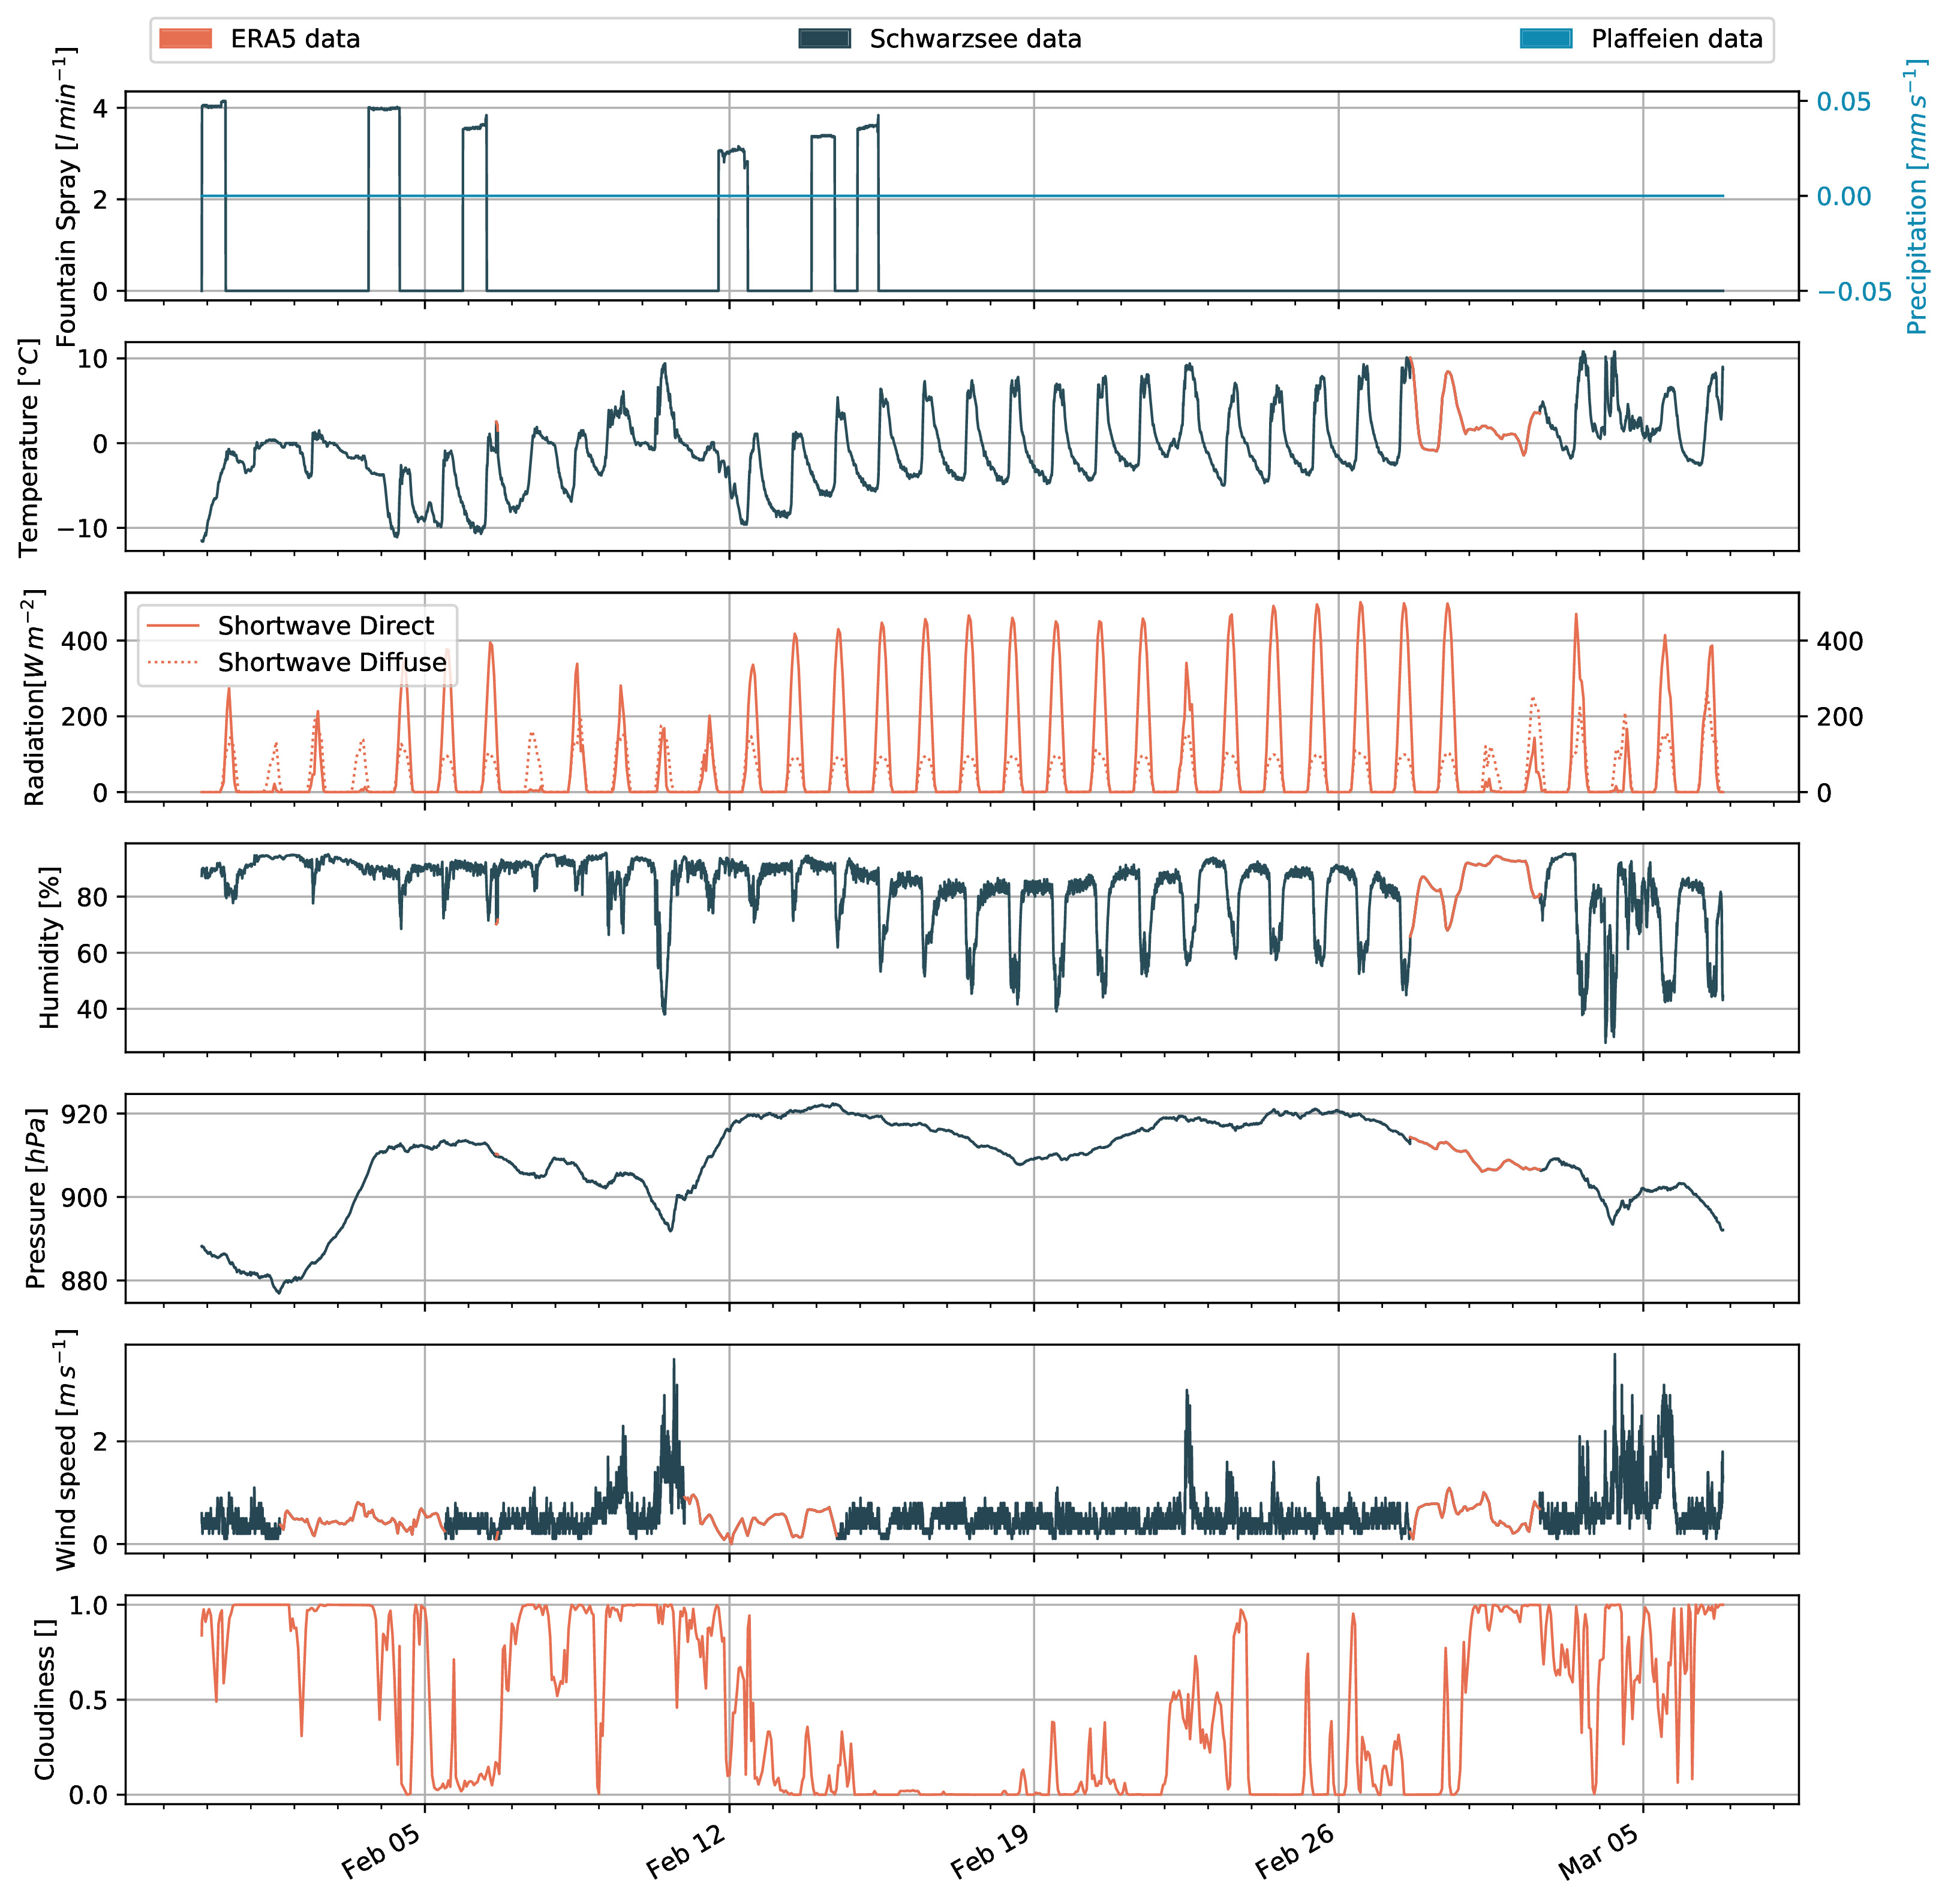
\includegraphics[width=\linewidth]{./Figures/Figure_3} \caption{Measurements at the AWS of
    EP were used as main model input data in 5 minute frequency. Plaffeien AWS provided the precipitation data.
    Incoming shortwave and longwave radiation were obtained from ERA5 reanalysis dataset. Several data gaps and errors
    were also filled from the ERA5 dataset (shaded regions).} \label{fig:input} \end{figure}

Due to a power failure, all data from the EP AWS was lost between $27^{th}$ February 15:20 2019 to $2^{nd}$ March 15:00
2019. Consequently, the amount of missing data in the dataset was around 7\%.  During heavy snowfall events, the
ultrasonic wind sensor was blocked and recorded zero values. ERA5 was used to fill such errors and data gaps .
Near-surface humidity is not archived directly in ERA datasets, but from near-surface ($2\,m$ from the surface)
temperature ($T_{ERA5}$) and dew point temperature ($Tw_{ERA5}$) one can calculate relative humidity($RH$) at $2\,m$ as
follows: \begin{equation} RH = 100 \cdot \frac{e_{sat}(Tw_{ERA5})}{e_{sat}(T_{ERA5})} \end{equation} where the
saturation vapour pressure function $e_{sat}$ is expressed with the Teten's formula \citep{Tetens}: \begin{equation}
e_{sat}(T)= a_1 \cdot e^{(a_3 \cdot \frac{T}{(T+273.16-a_4)})} \end{equation} with T in $\degree C$ and the parameters
set for saturation over water ($a_1$ = 611.21 Pa, $a_3$ = 17.502 and $a_4$= 32.19 K) according to \cite{Buck_1981}.
Zero wind speed values were recorded whenever snow accumulated on the ultrasonic wind sensor. So all null values were
replaced using the ERA5 dataset. 

The ERA5 grid point chosen (Latitude 46° 38' 24" N, Longitude 7° 14' 24" E) for the EP site was around 9 km
away from the actual site.  So all the ERA5 variables were fitted with the Schwarzee dataset via linear regressions.
Through this modified ERA5 dataset, we were also able to further extend the EP dataset and allow the model to
run beyond $18^{th}$ March 2019. Precipitation was filled as null values beyond $18^{th}$ March 2019.


\subsubsection{Field Measurements for validation} \label{section:validation} 
The volume was determined by decomposing the ice structure into a cylinder (length $2R$ and height $h$) and a
cone (radius $r$ and height $(H_i-h)$) through the following equation: 
\begin{equation} V = \pi \cdot R^2 \cdot h + 1/3 \cdot \pi \cdot r^2 \cdot (H_i-h) \end{equation}

Manual measurements were performed at the end of the freezing period on $14^{th}$ February 16:00 2019 (only one more
fountain run was possible after this date) to estimate $r, R, h, H_i, H_f$ (see Fig. \ref{fig:site} for the different
geometry components):

$$ 0.55\leq r\leq 1 m\textit{ ; }1.1\leq R\leq 1.2 m\textit{ ; }0.1\leq h\leq 0.2 m\textit{ ; }0.6\leq
H_i\leq 0.8 m\textit{ ; }1.3\leq H_f\leq 1.4 m  $$

The ranges of the variables show its variance across different compass orientations.  Correspondingly, the volume range
estimated for the first validation point was 0.857 $\pm$ 0.186 $m^{3}$ on $14^{th}$ February 16:00 2019.

The second validation point corresponds to the end of the melting process on $10^{th}$ March 18:00 2019.  Based on the
webcam imagery and manual measurement, a thin layer of ice with an observed thickness between 0.01 to 0.06 m could be
quantified. This results in the volume range for the second validation to be 0.13 $\pm$ 0.09 $m^{3}$ on $11^{th}$ March
2019 

In reality, the EP ice structure was more cylindrical until a height of 0.2\,$m$ and conical afterwards until a
height of 0.6\,$m$ with a radius of 1.18\,$m$. However, we assume a conical shape of this ice structure in order to
apply the modelling strategy described below.

\section{Model setup}

The model (implemented in python) consists of three parts calculating a) the geometric evolution of the Icestupa, b)
the energy balance and c) the mass balance as shown schematically in Fig. \ref{fig:schema}. A bulk energy and mass
balance model is used to calculate the amounts of ice, liquid water, water vapour and runoff water of the Icestupa
every 5 minutes. The equations used henceforth display model time step superscript only if it is different from the
current time step.

  \begin{figure} \begin{center} 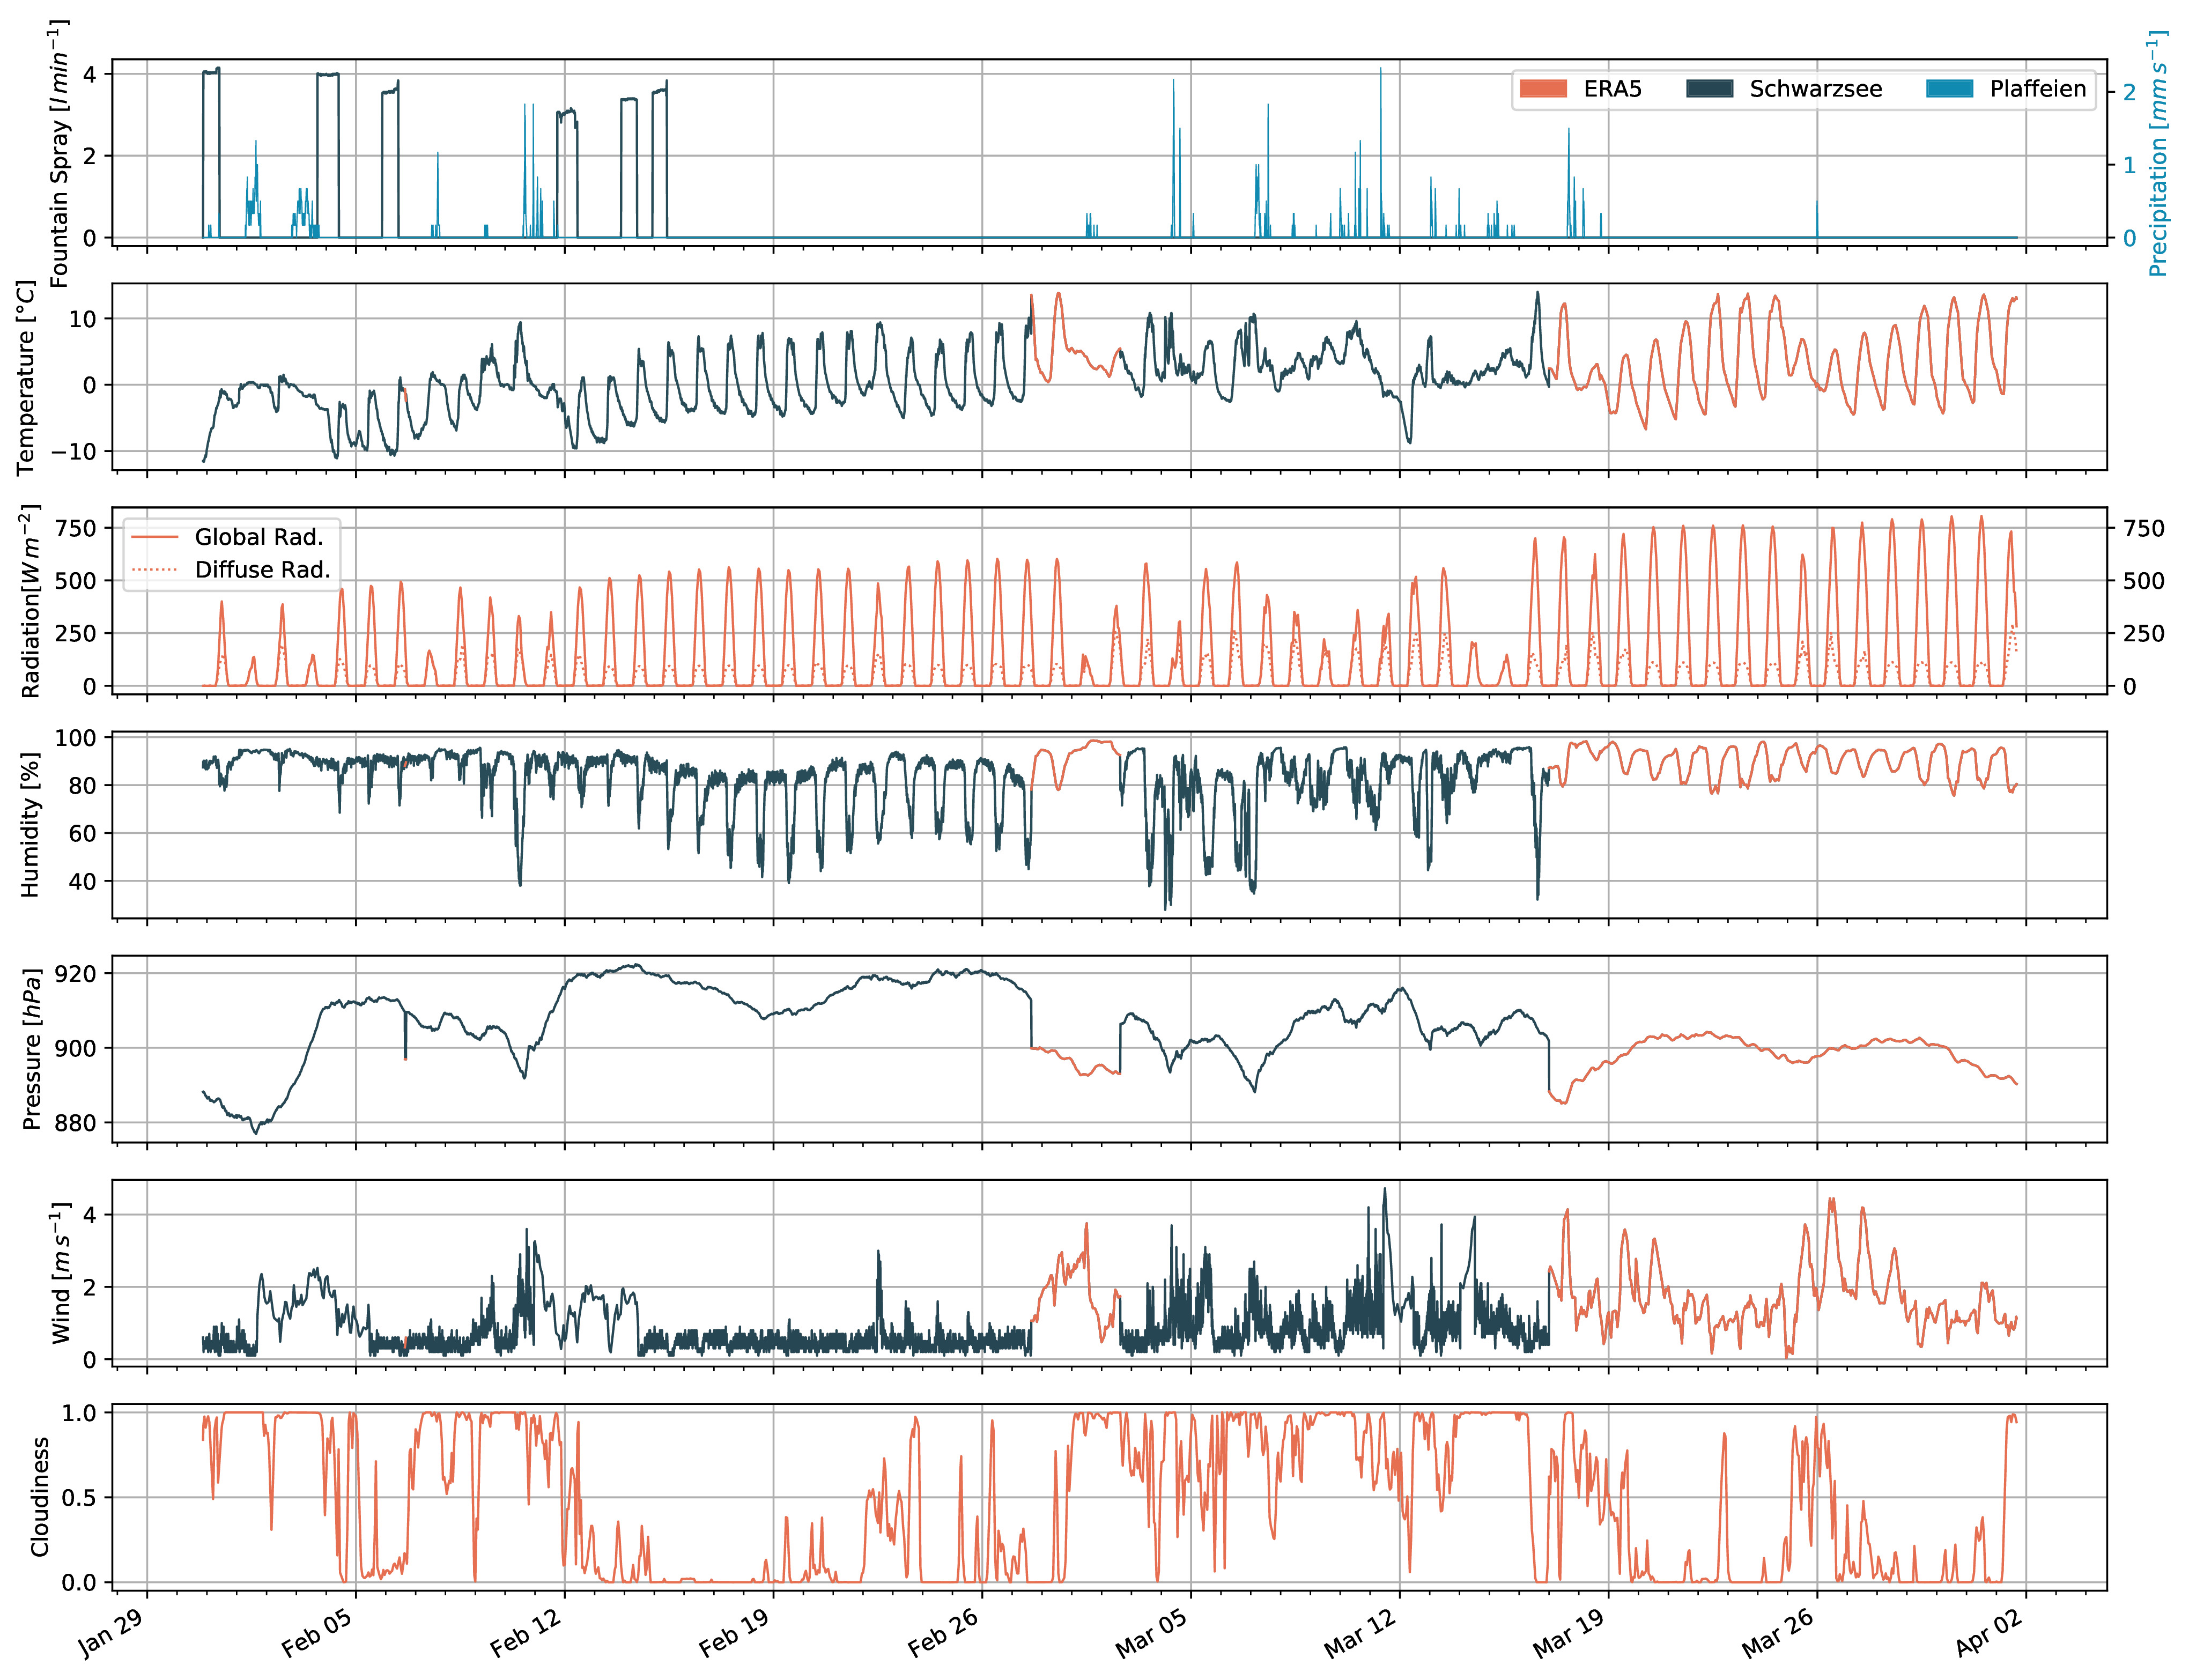
\includegraphics[width=15 cm]{Figures/Figure_4.jpg} \end{center} \caption{Model
schematic showing the algorithm used in the model at every time step. Further details about these variables can be
found in the associated tables and figures.} \label{fig:schema} \end{figure}

\subsection{Icestupa geometric evolution}

Radius $r_{ice}$ and height $h_{ice}$ define the dimensions of the Icestupa assuming its geometry to be a cone as
shown in Fig. \ref{fig:shape}. The surface area $A$ exposed to the atmosphere and volume $V$ are:

\begin{equation} A = \pi \cdot r_{ice} \cdot \sqrt{{r_{ice}}^2 + {h_{ice}}^ 2} \label{eqn:A} \end{equation}

\begin{equation} V = \pi/3 \cdot {r_{ice}}^2 \cdot h_{ice} \label{eqn:V} \end{equation}

With the mass of the Icestupa $M_{ice}$, its current volume can also be expressed as:

\begin{equation} V = M_{ice} / \rho_{ice} \label{eqn:V1} \end{equation}

where $\rho_{ice}$ is the density of ice (917 $kg\, m^{-3}$). The model of the Icestupa is initialised with a
thickness of $\Delta x$ (defined in \ref{section:EB}) and a circular area of radius $r_F$. The constant $r_F$
represents the mean spray radius of the fountain.  This fountain spray radius is determined by modelling the
projectile motion of the water droplets. Using mass conservation the droplet speed $v_F$ can be determined from the
spray rate $d_F$ and the diameter $dia_F$ of the nozzle as follows:

\begin{equation} v_F = \frac{d_F}{\pi \cdot dia_F^2/4} \end{equation}

Afterwards, we assume that the water droplets move with an air friction free projectile motion from the fountain
nozzle with a height $h_F$ to the ice/ground surface. The resulting spray radius $r_F$ was then determined from the
projectile motion equation as follows:

\begin{equation} r_F = \frac{v_F \cdot cos\theta_F (v_F \cdot sin\theta_F + \sqrt{(v_F \cdot sin\theta_F)^{2} + 2
\cdot g \cdot h_F})}{g} \end{equation}

where $g = 9.8 m s^{-2}$ is the acceleration due to gravity and $\theta_F$ = 45 $\degree$ is the angle of launch.

During subsequent time steps, the dimensions of the Icestupa evolve assuming a uniform ice formation and decay across
its surface area with an invariant slope $s_{cone} = \frac{h_{ice}}{r_{ice}}$ as shown in Fig.  \ref{fig:shape}.
During these time steps, the volume is parameterised using Eqn. \ref{eqn:V} as:

\begin{equation} V = \pi/3 \cdot {r_{ice}}^3 \cdot s_{cone} \label{eqn:V2} \end{equation}

  \begin{figure} \begin{center} 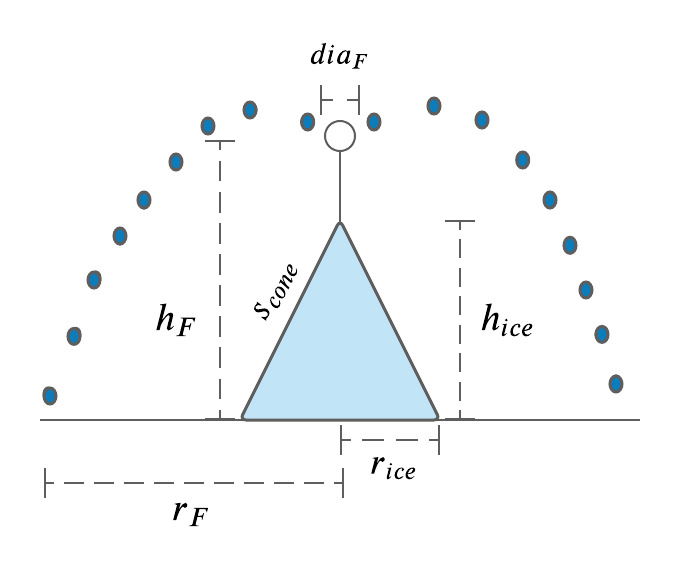
\includegraphics[width=10 cm]{Figures/Figure_5.jpg} \end{center} \caption{Shape and
fountain parameters of the EP Icestupa. $r_{ice}$ is the radius, $h_{ice}$ is the height and $s_{cone}$ is the
slope of the ice cone. $r_F$ is the spray radius, $h_F$ is the height and $dia_F$ is the nozzle diameter of the
fountain.} \label{fig:shape} \end{figure}
  
However, the Icestupa cannot outgrow the maximum range of the water droplets ($(r_{ice})_{max} = r_{F}$). Combining
equations \ref{eqn:V}, \ref{eqn:V1} and \ref{eqn:V2}, the geometric evolution of the Icestupa at each time step $i$
can be determined by considering the following rules:

\begin{equation} (r_{ice},\, h_{ice}) = \left\{ \begin{array}{ll} (r_F ,\, \Delta x) & \textit{ if } i=0\\
    (r_{ice}^{i-1},\, \frac{3 \cdot M_{ice}}{\pi \cdot \rho_{ice} \cdot {(r_{ice}^{i-1})}^2}) & \textit{ if }
    r_{ice}^{i-1} \geq r_{F} \textit{ and } \Delta M_{ice} > 0 \textit{ where } \Delta M_{ice} = M_{ice}^{i-1} -
    M_{ice}^{i-2}\\ (\frac{3 \cdot M_{ice}}{\pi \cdot \rho_{ice} \cdot s_{cone}})^{1/3} \cdot (1,\,  s_{cone}) &
otherwise \end{array} \right.  \label{eqn:A2} \end{equation}

\subsection{Energy Balance} \label{section:EB}

The energy balance equation \citep{Hock_2005} for the Icestupa is formulated as follows:

\begin{equation} q_{net} = q_{SW} + q_{LW} + q_{L} + q_{S} + q_{F} + q_{G} \label{eqn:EF} \end{equation}

where $q_{net}$ is the net energy flux in [$W\,m^{-2}$]; $q_{SW}$ is the net shortwave radiation; $q_{LW}$ is the net
longwave radiation; $q_{L}$ and $q_{S}$ are the turbulent latent and sensible heat fluxes. $q_{F}$ represents the heat
exchange of the fountain water droplets with the AIR ice surface during fountain on time steps. $q_{G}$
represents ground heat flux between Icestupa surface and Icestupa interior. Energy transferred in the direction of the
ice surface is always denoted as positive and away as negative.  

Equation \ref{eqn:EF} is usually referred to as the energy budget for “the surface”, but practically it must apply to
a surface layer of ice with a finite thickness $\Delta x$. The energy flux acts upon the Icestupa surface layer which
has an upper and a lower boundary defined by the atmosphere and the ice body of the Icestupa, respectively. The
parameter selection for $\Delta x$ is based on the following two arguments: (a) the ice thickness $\Delta x$ should be
small enough to represent the daily surface temperature variations and (b) $\Delta x$ should be large enough for these
temperature variations to not reach the bottom of the surface layer.  Therefore, we introduced a 5 $mm$ thick ice
surface layer, over which the energy balance is calculated. A sensitivity analysis was later performed to understand
the influence of this factor. Here, we define the surface temperature $T_{ice}$ to be the modelled average temperature
of the Icestupa surface layer and the energy flux $q_{net}$ is assumed to act uniformly across the Icestupa area $A$.

\subsubsection{Net Shortwave Radiation $q_{SW}$} The net shortwave radiation $q_{SW}$ is computed as follows:
\begin{equation} q_{SW} = (1- \alpha)\cdot (SW_{direct} \cdot f_{cone} + SW_{diffuse}) \label{eqn:SW} \end{equation}

where $SW_{direct}$ and $SW_{diffuse}$ are the ERA5 direct and diffuse short wave radiation, $\alpha$ is the modelled
albedo and $f_{cone}$ is the area fraction of the ice structure exposed to the direct shortwave radiation.

We model the albedo using a scheme described in \cite{OerlemansKnap_1998}. The scheme records the decay of albedo with
time after fresh snow is deposited on the surface. $\delta t$ records the number of time steps after the last snowfall
event. After snowfall, albedo changes over a time step, $\delta t$ , as

\begin{equation} \alpha=\alpha_{ice}+(\alpha_{snow}-\alpha_{ice}) \cdot e^{(-\delta t)/\tau} \label{eqn:a}
\end{equation}

where $\alpha_{ice}$ is the bare ice albedo value (0.35), $\alpha_{snow}$ is the snow ice albedo value (0.85) and
$\tau$ is a decay rate, which determines how fast the albedo of the ageing snow reaches this value.  The decay rate
$\tau$ is assumed to have a base value of 10 days similar to values obtained by \cite{Schmidt_2017} for wet surfaces
and its maximal value is set based on observations by \cite{OerlemansKnap_1998} as shown in Table
\ref{table:parameters}.  Furthermore, the albedo $\alpha$ varies depending on the water source that formed the current
Icestupa surface.  Correspondingly, the albedo is reset to the value of bare ice albedo if the fountain is spraying
water onto the current ice surface and to the value of fresh snow albedo if a snowfall event occurred. Snowfall events
are assumed if the air temperature is below $T_{ppt}=1 \degree C$ \citep{FujitaAgeta_2000}.

The area fraction $f_{cone}$ of the ice structure exposed to the direct shortwave radiation depends on the shape
considered. The direct solar radiation incident on the AIR surface is first decomposed into horizontal and vertical
components using the solar elevation angle $\theta_{sun}$. For a conical shape, half of the total curved surface is
exposed to the vertical component of the direct shortwave radiation and the projected triangle of the curved surface is
exposed to the horizontal component of the direct shortwave radiation. The solar elevation angle $\theta_{sun}$ used is
modelled using the parametrisation proposed by \cite{Woolf_1968}. Accordingly, $f_{cone}$ is determined as follows:

\begin{equation} \begin{split} f_{cone}& =\frac{(0.5 \cdot r_{ice} \cdot h_{ice}) \cdot cos \theta_{sun} +(\pi \cdot
{r_{ice}}^2/2) \cdot sin \theta_{sun} }{\pi \cdot r_{ice} \cdot ({r_{ice}}^2+{h_{ice}}^2)^{1/2}}\\ \end{split}
\label{eqn:f_{cone}} \end{equation}

The measured diffuse shortwave radiation is assumed to impact the conical Icestupa surface uniformly. 

\subsubsection{Net Longwave Radiation $q_{LW}$}

The net longwave radiation $q_{LW}$, for which there were no direct measurements available at EP, is
determined as follows:

\begin{equation} q_{LW}= LW_{in}-\sigma \cdot \epsilon_{ice} \cdot {(T_{ice}+ 273.15)}^4
\label{eqn:LW} \end{equation}

where $T_a$ represents the measured air temperature, $T_{ice}$ is the modelled surface temperature, both temperatures
are given in [$\degree C$], $\sigma=5.67 \cdot 10^{−8}\,Jm^{-2}s^{-1}K^{-4}$ is the Stefan-Boltzmann constant,
$LW_{in}$
denotes the incoming longwave radiation derived from the ERA5 dataset and $\epsilon_{ice}$ is the corresponding
emissivity value for the Icestupa surface (see Table \ref{table:parameters}).

\subsubsection{Turbulent sensible $q_{S}$ and latent $q_{L}$ heat fluxes }

The turbulent sensible $q_{S}$ and latent heat $q_{L}$ fluxes are computed with the following expressions proposed by
\cite{Garratt_1992}:

\begin{equation} q_{S}=c_{a} \cdot \rho_{a} \cdot p_{a}/p_{0,a} \cdot \frac{\kappa^2 \cdot v_a \cdot
(T_a-T_{ice})}{{(\ln{\frac{h_{AWS}}{z_{ice}}})}^2} \label{eqn:qs} \end{equation}

\begin{equation} q_{L}=0.623 \cdot L_s \cdot \rho_{a}/p_{0,a} \cdot \frac{\kappa^2 \cdot
         v_a(p_{v,a}-p_{v,ice})}{{(\ln{\frac{h_{AWS}}{z_{ice}}})}^2}
\end{equation}

where $h_{AWS}$ is the measurement height above the ground surface of the AWS (in $m$), $v_a$ is the wind speed in
[$m\,s^{-1}$] and $M_{F}$ denotes fountain water spray mass in [$kg$]. $c_a$ is the specific heat of air at constant
pressure (1010 J $kg^{-1} K^{-1}$), $\rho_{a}$ is the air density at standard sea level (1.29 $kg m^{-3}$), $p_{0,a}$
is the air pressure at standard sea level (1013 $hPa$), $\kappa$ is the von Karman constant (0.4), $L_s$ is the heat
of sublimation (2848 $kJ\, kg^{-1}$) and $z_{ice}$ (1.7 $mm$) denotes the roughness length of ice (momentum and
scalar) described in \citep{Garratt_1992}.The vapor pressures over air ($p_{v,a}$) and ice ($p_{v,ice}$) was obtained using the following formulation given in \cite{WMO_2018}:

\begin{equation} \begin{split} p_{v,a}&=6.107 \cdot 10^{(7.5 \cdot T_a / (T_a + 237.3))}\\ p_{v,ice}&=(1.0016 +
3.15\cdot10^{-6}\cdot p_{a}-0.074\cdot p_{a}^{-1})\cdot(6.112 \cdot e^{(22.46 \cdot T_{ice} / (T_{ice} + 272.62))})
\end{split} \label{eqn:vp} \end{equation}

where $p_{a}$ is the measured air pressure in [$hPa$]. 
\subsubsection{Fountain water heat flux $q_{F}$ }

The total energy flux is further influenced through the heat flux caused by the water that was additionally added to
the surface of the Icestupa during the time the fountain was running. We take this interaction between the fountain
water and the ice surface into account by assuming that the ice surface temperature stays constantly at 0 $\degree C$
during time steps when the fountain is active. This process can be divided into two simultaneous steps: (a) the water
temperature $T_{water}$ is cooled to 0 $\degree C$ and (b) the ice surface temperature is warmed to 0 $\degree C$.
Process (a) transfers hereby the necessary energy for process (b) throughout the fountain runtime. We further assume
that this process is instantaneous, i.e. the ice temperature is immediately set to 0 $\degree C$ within just one time
step $\Delta t$ when the fountain is switched on. Thus, the heat flux caused by the fountain water is calculated as
follows:

\begin{equation} 
  q_{F} = \left\{ \begin{array}{ll}
         0 & \textit{ if } \Delta M_{F} = 0\\ \frac{ \Delta M_F \cdot c_{water} \cdot T_{water}}{\Delta t \cdot A} +
         \frac{\rho_{ice} \cdot \Delta x \cdot c_{ice} \cdot T_{ice}}{\Delta t} & \textit{ if } \Delta M_{F} > 0 
    \end{array} \right.  \label{eqn:qF}
\end{equation} 
with $c_{ice}$ as the specific heat of ice. 

\subsubsection{Bulk Icestupa heat flux $q_{G}$} \label{sec:Bulkflux}
The bulk Icestupa heat flux $q_{G}$ corresponds to the ground heat flux in normal soils and is caused by the
temperature gradient between the surface layer and the ice body. It is expressed by using the heat conduction equation
as follows:

\begin{equation} q_{G} = k_{ice} \cdot (T_{bulk}-T_{ice})/l_{ice} \label{eqn:qG}    \end{equation}

where $k_{ice}$ is the thermal conductivity of ice in [$W\, m^{-1}\,K^{-1}$] , $T_{bulk}$ is the mean temperature of
the ice body within the Icestupa and $l_{ice}$ is the average distance of any point in the surface to any other point
in the ice body. $T_{bulk}$ is initialised as 0 $\degree C$ and later determined from Eqn. \ref{eqn:qG} as follows:

\begin{equation} T_{bulk} = T_{bulk}^{i-1} - (q_{G} \cdot A \cdot \Delta t)/(M_{ice} \cdot c_{ice}) \end{equation}

Since we assume a conical shape with $r_{ice} > h_{ice}$, $l_{ice}$ cannot be greater than $2r_{ice}$ and also cannot
be less than $\Delta x$. Therefore, the average distance from any point on the surface to any point inside is $\Delta
x \leq l_{ice} \leq r_{ice}$. We calculate $q_{G}$ here assuming $l_{ice} = r_{ice}/2$.


\subsubsection{Surface temperature changes and melt energy $q_{melt}$}
The available net energy $q_{net}$ partly increases surface temperature, but also contributes to ice melt at the
surface of the Icestupa. $q_{T}$ denotes the energy used on changing the surface temperature $T_{ice}$ and $q_{melt}$
denotes the energy used to produce meltwater. So Eqn. \ref{eqn:EF} can be rewritten as: \begin{equation} q_{net} =
q_{melt} + q_{T} \end{equation}

We define the freezing energy as $q_{freeze} = (q_{net}-q_{L})$. This is because the latent heat always contributes to
temperature fluctuations. Now, the temperature fluctuates based on 3 scenarios namely, (1) the freezing energy flux is
negative but cannot freeze all the fountain water output; (2) the freezing energy flux is negative and can freeze all
the fountain water output; (3) the freezing energy is positive and (4) the fountain is inactive ($\Delta M_{F}=0$).
Therefore, we express the rate of change of temperature as follows:

\begin{equation} \frac{\Delta T}{\Delta t} = \left\{ \begin{array}{ll} -T_{ice}^{i-1}/\Delta t & \textit{ if }
     q_{freeze} < 0 \textit{ and } \Delta M_{F} \geq -q_{freeze}\cdot A \cdot \Delta t/L_f  \\ (\Delta M_{F}
    \cdot L_f )/(\rho_{ice} \cdot c_{ice} \cdot  \Delta x \cdot A \cdot \Delta t) & \textit{ if }  q_{freeze}< 0
    \textit{ and } \Delta M_{F} < -q_{freeze}\cdot A \cdot \Delta t/L_f  \\ q_{net}/ (\rho_{ice}\cdot c_{ice}
    \cdot \Delta x)& \textit{ if } \Delta M_{F} = 0 \textit{ or }  q_{freeze}> 0
    \end{array} \right.  \label{eqn:T} \end{equation}
Whenever the model predicts $T_{ice}^{i+1} > 0 \degree C$, then the surface temperature is set to 0 $\degree C$ in the
corresponding time step and additional energy contributes to $q_{melt}$. Combining these requirements, we get:

\begin{equation} (q_{T}, q_{melt}) = \left\{ \begin{array}{ll} ( \rho_{ice} \cdot c_{ice} \cdot  \Delta x \cdot
    \frac{\Delta T}{\Delta t}, q_{net}-q_{L}-\rho_{ice} \cdot c_{ice} \cdot  \Delta x \cdot \frac{\Delta T}{\Delta t})
    & \textit{ if } T_{ice}^{i+1}\leq 0 \degree C \textit{ and } \Delta M_{F} > 0\\ ( \rho_{ice} \cdot c_{ice} \cdot  \Delta x
    \cdot \frac{\Delta T}{\Delta t}, q_{net}-\rho_{ice} \cdot c_{ice} \cdot  \Delta x \cdot \frac{\Delta T}{\Delta t})
    & \textit{ if } T_{ice}^{i+1}\leq 0 \degree C \textit{ and } \Delta M_{F} = 0\\
        ( -\rho_{ice} \cdot c_{ice} \cdot  \Delta x \cdot \frac{T_{ice}^{i}}{\Delta t}, q_{net}-q_{L}+\rho_{ice} \cdot
    c_{ice} \cdot \Delta x \cdot \frac{T_{ice}^{i}}{\Delta t}) & \textit{ if } T_{ice}^{i+1}> 0 \degree C \textit{ and } \Delta
    M_{F} > 0\\ ( -\rho_{ice} \cdot c_{ice} \cdot  \Delta x \cdot \frac{T_{ice}^{i}}{\Delta t}, q_{net}+\rho_{ice}
    \cdot c_{ice} \cdot  \Delta x \cdot \frac{T_{ice}^{i}}{\Delta t}) & \textit{ if } T_{ice}^{i+1}> 0 \degree C \textit{ and }
\Delta M_{F} = 0\\ \end{array} \right.  \label{eqn:qt} \end{equation}

\begin{table*}[p] \caption{Free parameters in the model categorised as constant, uncertain and site parameters. Base
  value (B) and uncertainty (U) were taken from the literature. For assumptions (assum.), the uncertainty was chosen
to be relatively large (5 \%). For measurements (meas.), the uncertainty due to parallax errors is chosen to be (1
\%).}
    
    \begin{tabularx}{\linewidth}{ X l X l X  } \hline Constant Parameters & Symbol & Value & & References \\ \hline Van
      Karman constant & $\kappa$ & 0.4 &  & B: \citeauthor{CuffeyPaterson_2010}\\ Stefan Boltzmann constant & $\sigma$
                      & $5.67 \cdot 10^{-8} W\, m^{-2}\, K^{-4}$&  & B: \citeauthor{CuffeyPaterson_2010}\\ Air pressure
      at sea level & $p_{0,a}$ & 1013 $hPa$ &  & B: \citeauthor{MolgHardy_2004}\\ Density of water & $\rho_{w}$ & 1000
      $kg\, m^{-3}$ &    & B: \citeauthor{CuffeyPaterson_2010}\\ Density of ice & $\rho_{ice}$ & 917 $kg\, m^{-3}$ &
                    & B: \citeauthor{CuffeyPaterson_2010}\\ Density of air & $\rho_{a}$ &  1.29 $kg\, m^{-3}$ &   & B:
      \citeauthor{MolgHardy_2004}\\ Specific heat of water & $c_{w}$ & 4186 $J\, kg^{-1}\,\degree C^{-1}$ &   & B:
      \citeauthor{CuffeyPaterson_2010}\\ Specific heat of ice & $c_{ice}$ & 2097 $J\, kg^{-1}\,\degree C^{-1}$ &    &
      B: \citeauthor{CuffeyPaterson_2010}\\ Specific heat of air & $c_{a}$ & 1010 $J\, kg^{-1}\,\degree C^{-1}$ &   &
      B: \citeauthor{MolgHardy_2004}\\ Thermal conductivity of ice & $k_{ice}$ & 2.123  $W\, m^{-1}\, K^{-1}$ &  & B:
      \citeauthor{Bonales_2017} \\ Latent Heat of Sublimation & $L_{s}$ & 2848 $kJ\, kg^{-1}$ &    & B:
      \citeauthor{CuffeyPaterson_2010}\\ Latent Heat of Evaporation & $L_{e}$ & 2514 $kJ\, kg^{-1}$ &    & B:
      \citeauthor{CuffeyPaterson_2010}\\ Latent Heat of Fusion & $L_{f}$ & 334 $kJ\, kg^{-1}$ &    & B:
      \citeauthor{CuffeyPaterson_2010}\\ Gravitational acceleration & $g$ & 9.81 $m\, s^{-2}$ &    & B:
      \citeauthor{CuffeyPaterson_2010}\\ \hline Uncertain Parameters& & & Range   & \\ \hline Precipitation Temperature
      threshold & $T_{ppt}$ & 1 \degree C & $\pm$ $1\,\degree C$ & B + U: \citeauthor{FujitaAgeta_2000},
      \citeauthor{Zhou_2010}\\
        
        Ice Emissivity        & $\epsilon_{ice}$ & 0.95 & [0.949,0.993] 5 \% & B: \citeauthor{CuffeyPaterson_2010}; U:
        \citeauthor{HORI2006486}\\
        Ice Albedo         & $\alpha_{ice}$ & 0.35 & $\pm$ 5 \%  & B: \citeauthor{CuffeyPaterson_2010}; U: assum.   \\
        
        Snow Albedo        & $\alpha_{snow}$ & 0.85 & $\pm$ 5 \% & B: \citeauthor{CuffeyPaterson_2010}; U: assum.  \\
        Albedo Decay Rate & $\tau$ & 10 days & $[1,22]\, days$ & B: \citeauthor{Schmidt_2017}; U:
        \citeauthor{OerlemansKnap_1998}  \\ Ice layer thickness & $\Delta x$ & 5 $\,mm$ & $[1,10]\, mm$   & assum.\\
        % Ice body and surface distance & $l_{ice}$ & $r_{ice}/2$ & $[\Delta x, r_{ice}]\, mm$   & B + U: Section
        % \ref{sec:Bulkflux}\\
        
        \hline Site Parameters& & & & \\ \hline Fountain nozzle diameter & $dia_{F}$ & $5 \,mm$ & $\pm$ 1 $\%$   & B:
        meas. ; U: assum.\\ Fountain height & $h_{F}$ & $1.35 \,m$ &  $\pm$ 1 $\%$   & B: meas. ; U: assum.\\ Fountain
        water temperature & $T_{water}$ & 5 $\,\degree C$ & $[0,9] \,\degree C$   & B: meas. ; U: meas.\\ AWS height &
        $h_{AWS}$ & $3 \,m$ & $\pm$ 1 $\%$   & B: meas. ; U: assum.\\
        
        \hline \end{tabularx} \label{table:parameters} \end{table*} \clearpage

\subsection{Mass Balance} 
The mass balance equation is used to derive the water that drains away $M_{runoff}$ as follows:

\begin{equation} \frac{\Delta M_{runoff}}{\Delta t} = \frac{\Delta M_{F} + \Delta M_{ppt} + \Delta M_{dpt} - \Delta
M_{ice} -\Delta M_{melt} - \Delta M_{vapour}}{\Delta t} \label{eqn:M} \end{equation}
where $\Delta M = M^{i} - M^{i-1}$. Here $\frac{\Delta M_{F}}{\Delta t} = d_F$ where $d_F$ is the spray of the
fountain measured in [$kg\,s^{-1}$]; $M_{ppt}$ is the cumulative precipitation and $M_{dpt}$ is the
cumulative accumulation through water vapour condensation or deposition; $M_{ice}$ is the cumulative mass of ice;
$M_{melt}$ is the cumulative mass of melt water and $M_{vapour}$ represents the cumulative water vapor loss by
evaporation or sublimation. 

Precipitation input is calculated as:

\begin{equation} \frac{\Delta M_{ppt}}{\Delta t}  = \left\{ \begin{array}{ll} \pi \cdot {r_{ice}}^2 \cdot
\rho_{w}\cdot ppt& \textit{ if } T_{a} < T_{ppt} \\ 0 & \textit{ if } T_{a} \geq T_{ppt} \\ \end{array} \right.
    \end{equation}

where $\rho_{w}$ is the density of water (1000 $kg\,m^{-3}$), $ppt$ is the measured precipitation rate in
[$m\,s^{-1}$] and $T_{ppt}$ is the temperature threshold below which precipitation falls as snow. Here, snowfall
events were identified using $T_{ppt}$ as $1 \degree C$. Snow mass input is calculated by assuming a uniform
deposition over the entire circular footprint of the Icestupa. 

The latent heat flux is used to estimate either the evaporation and condensation processes or sublimation and deposition
processes.  To differentiate between these two possibilities, we classify the time steps into humid or non-humid if the
corresponding relative humidity value is above or below 60\% \citep{Stigter_2018}. On humid time steps we assume
condensation or evaporation to occur whereas on non-humid time steps deposition or sublimation can occur.
Correspondingly, latent heat of evaporation ($L_e$) is used for humid time steps and latent heat of sublimation ($L_s$)
is used for non-humid time steps. Water accumulation and vapour loss from the Icestupa surface is calculated as follows:

\begin{equation} (\frac{\Delta M_{vapour}}{\Delta t}, \frac{\Delta M_{dpt}}{\Delta t}) = \left\{ \begin{array}{ll}
(-q_{L} \cdot A /L,0) & \textit{ if } q_{L}<0 \\ (0,q_{L} \cdot A /L) & \textit{ if } q_{L}\geq0 \\ \end{array}
\right.  \label{eqn:vap} \end{equation}

where $ L = \left\{ \begin{array}{ll} L_s & \textit{ if } RH<60 \\ L_e & \textit{ if } RH\geq60\\  \end{array} \right.
$

Using the melt energy $q_{melt}$, we estimate the frozen and melted ice mass ($\Delta M_{ice}$, $\Delta M_{melt}$).
Removing the contribution of precipitation and combining Eqn. \ref{eqn:vap} we are left with the contribution from the
melt energy as follows:

\begin{equation} \left.\begin{aligned} (\frac{\Delta M_{ice}-\Delta M_{ppt}-\Delta M_{dpt} + \Delta M_{vapour}}{\Delta
    t},\\ \frac{\Delta M_{melt}}{\Delta t}) \textit{ if } RH < 60\\ (\frac{\Delta M_{ice}-\Delta M_{ppt}-\Delta
  M_{dpt}}{\Delta t}, \\ \frac{\Delta M_{melt}+ \Delta M_{vapour}}{\Delta t}) \textit{ if } RH \geq 60 \end{aligned}
\right\}= \left\{ \begin{array}{ll} \frac{q_{melt} \cdot A }{L_f} \cdot (-1, 1 )& \textit{ if } q_{melt} \geq 0 \\
\frac{q_{melt} \cdot A }{L_f} \cdot (-1, 0) & \textit{ if } q_{melt} < 0 \textit{ and } \frac{\Delta M_{F}}{\Delta t}
\geq -\frac{q_{melt} \cdot A }{L_f} \\
(\frac{\Delta M_{F}}{\Delta t}, 0) & \textit{ if } q_{melt} < 0 \textit{ and } 0 \leq
\frac{\Delta M_{F}}{\Delta t} < -\frac{q_{melt} \cdot A }{L_f}\\ \end{array} \right.  \end{equation}

Now, with all the other terms known in Eqn. \ref{eqn:M}, the water drainage/runoff can now be determined. 

Considering AIRs as water reservoirs, we can quantify their potential through the amount of water they store (storage
quantity) and the length of time they store it (storage duration). Another means of comparing different Icestupas is
through their water storage efficiency defined accordingly as:

\begin{equation} \textit{Storage Efficiency} = \frac{M_{melt}}{(M_F+M_{ppt}+M_{dpt})} \cdot 100 \end{equation}



\section{Model Results} 
The model was forced with meteorological data from $30^{th}$ January to $5^{th}$ April 2019 (Fig.
\ref{fig:input}) and various parameters (see Table \ref{table:parameters}) to calculate the mass and energy balance of
the Icestupa.

\begin{figure} \begin{center} 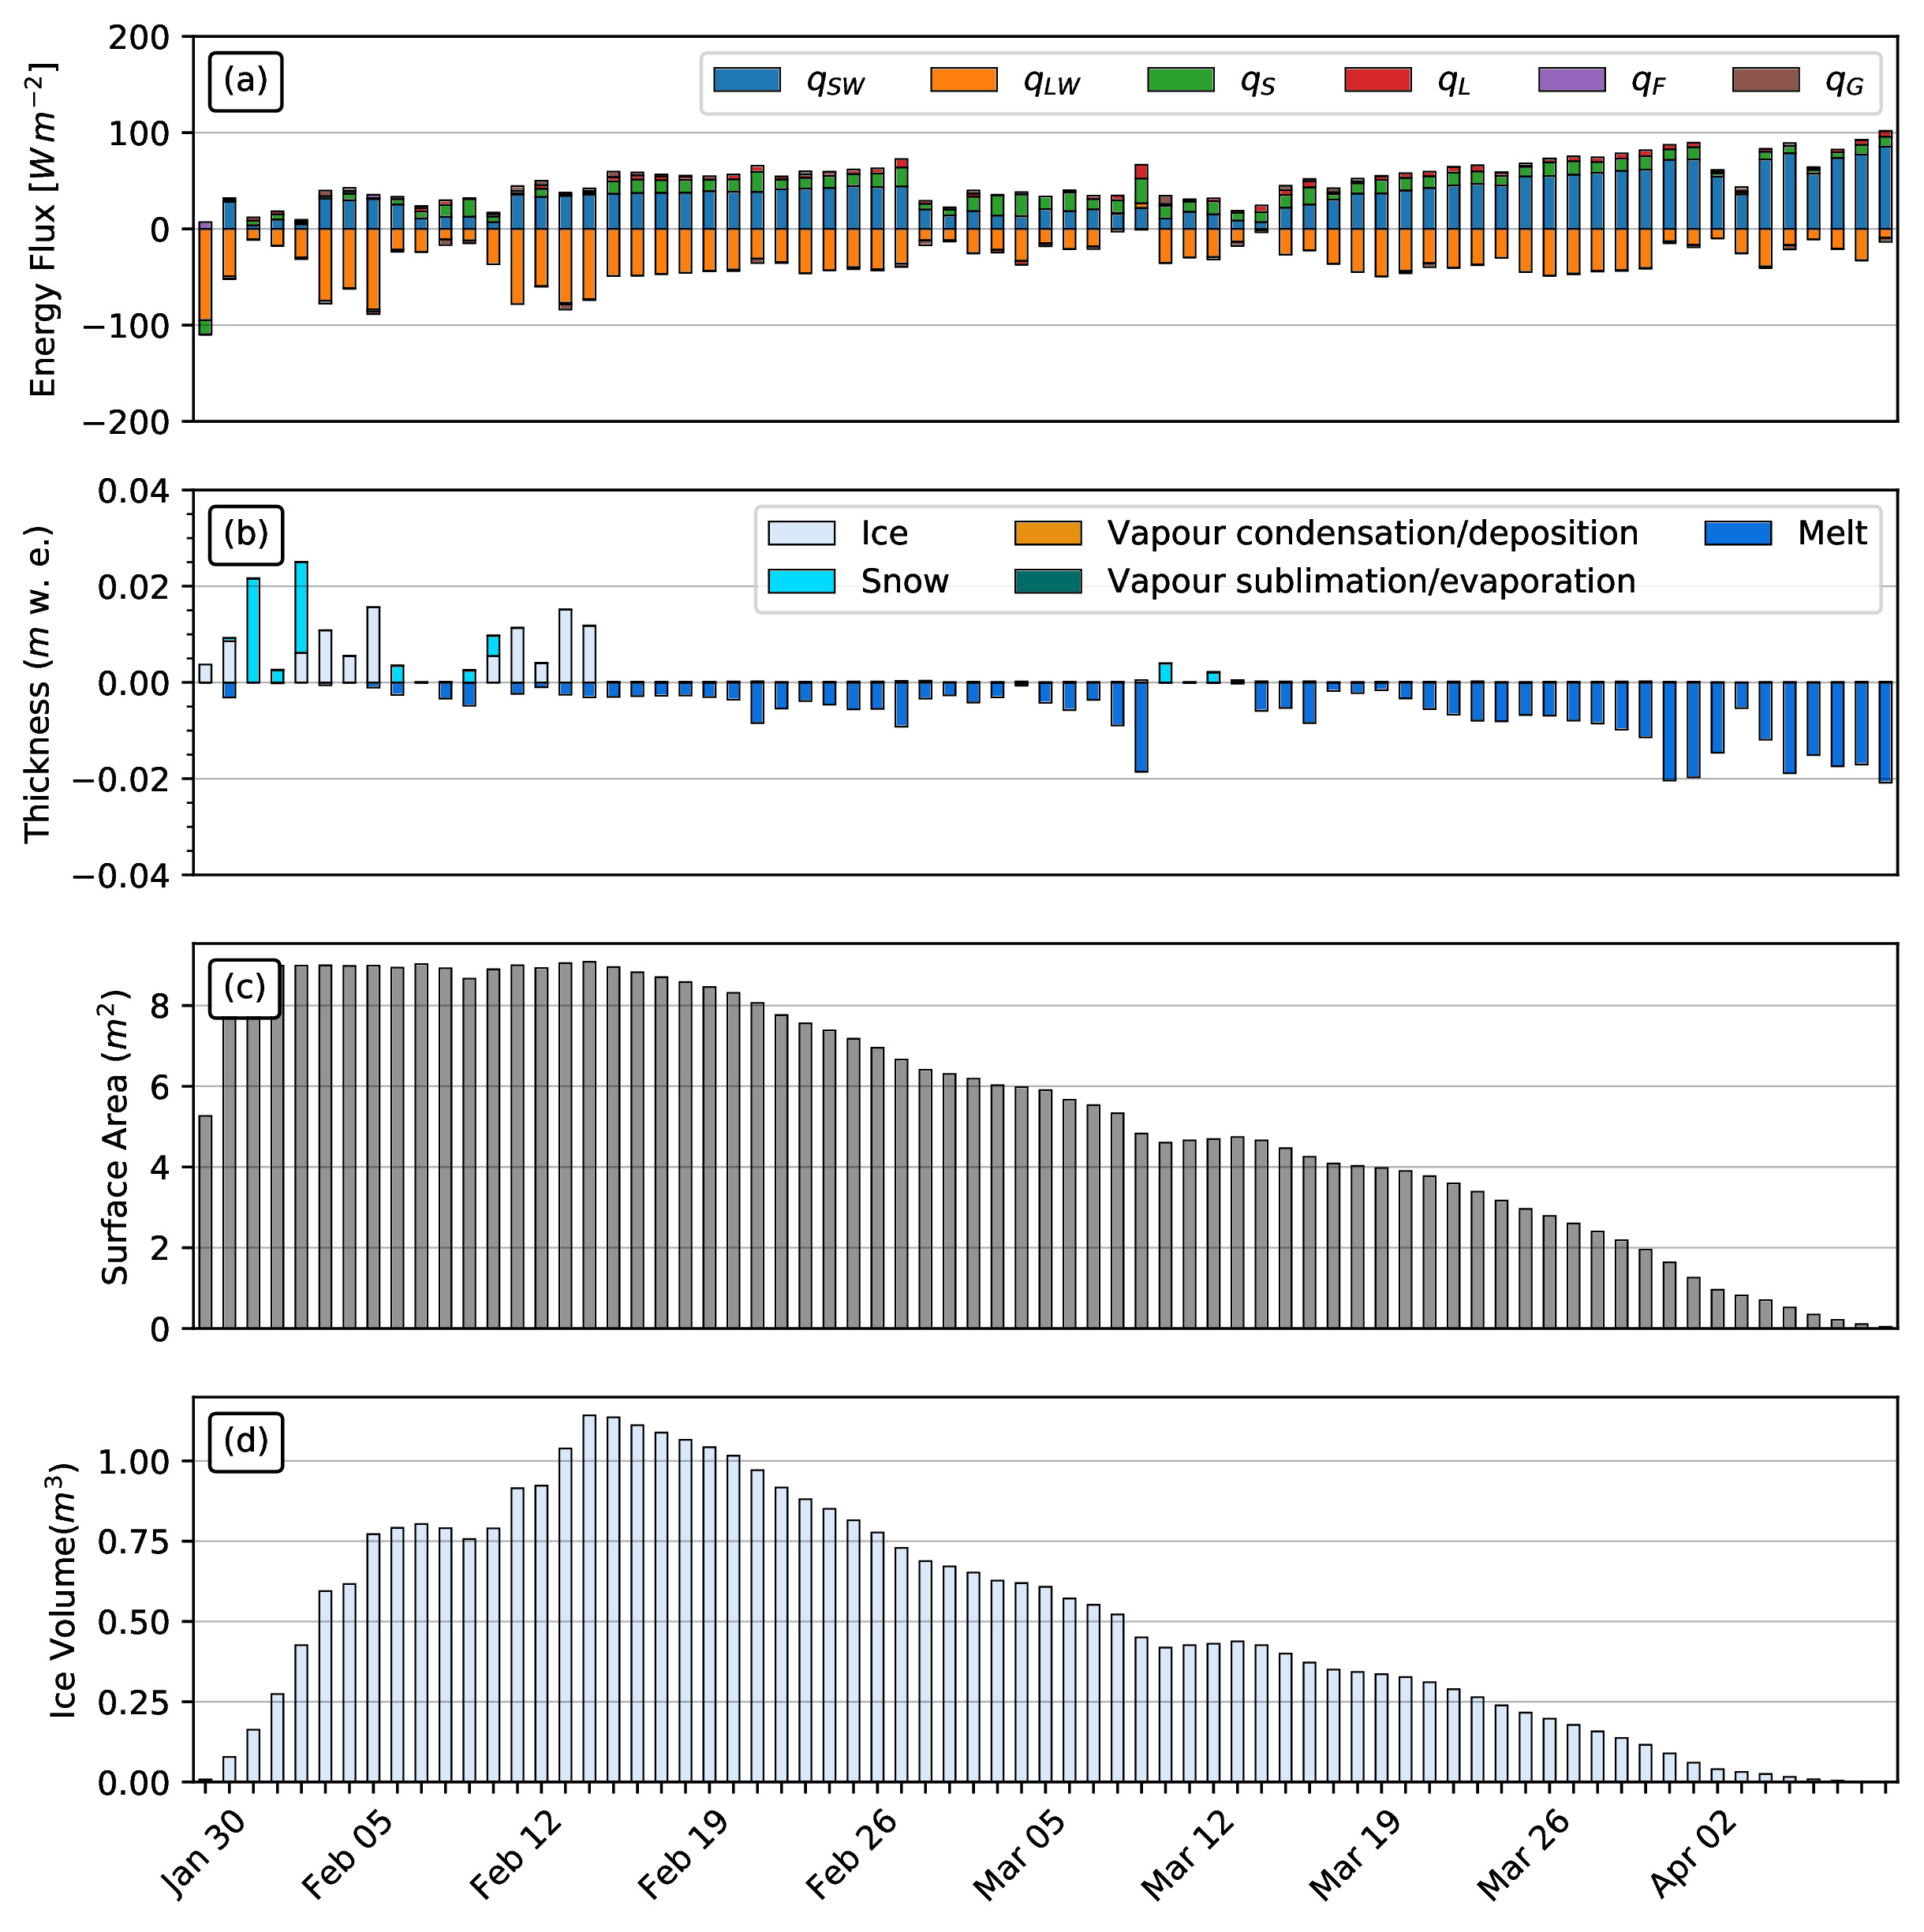
\includegraphics[width=\linewidth]{Figures/Figure_6.jpg} \end{center}
\caption{(a)Fountain discharge (b) energy flux components, (c) mass flux components (d) surface area and (e) volume of
  the Icestupa in daily time steps.  $q_{SW}$ is the net shortwave radiation; $q_{LW}$ is the net longwave radiation;
  $q_{L}$ and $q_{S}$ are the turbulent latent and sensible heat fluxes. $q_{F}$ represents the interactions of the
  ice-water boundary during fountain on time steps.  $q_{G}$ quantifies the heat conduction process between the
  Icestupa surface layer and the ice body. } \label{fig:EB} \end{figure} \subsection{Energy and mass balance
calculation}

\begin{figure} \begin{center} 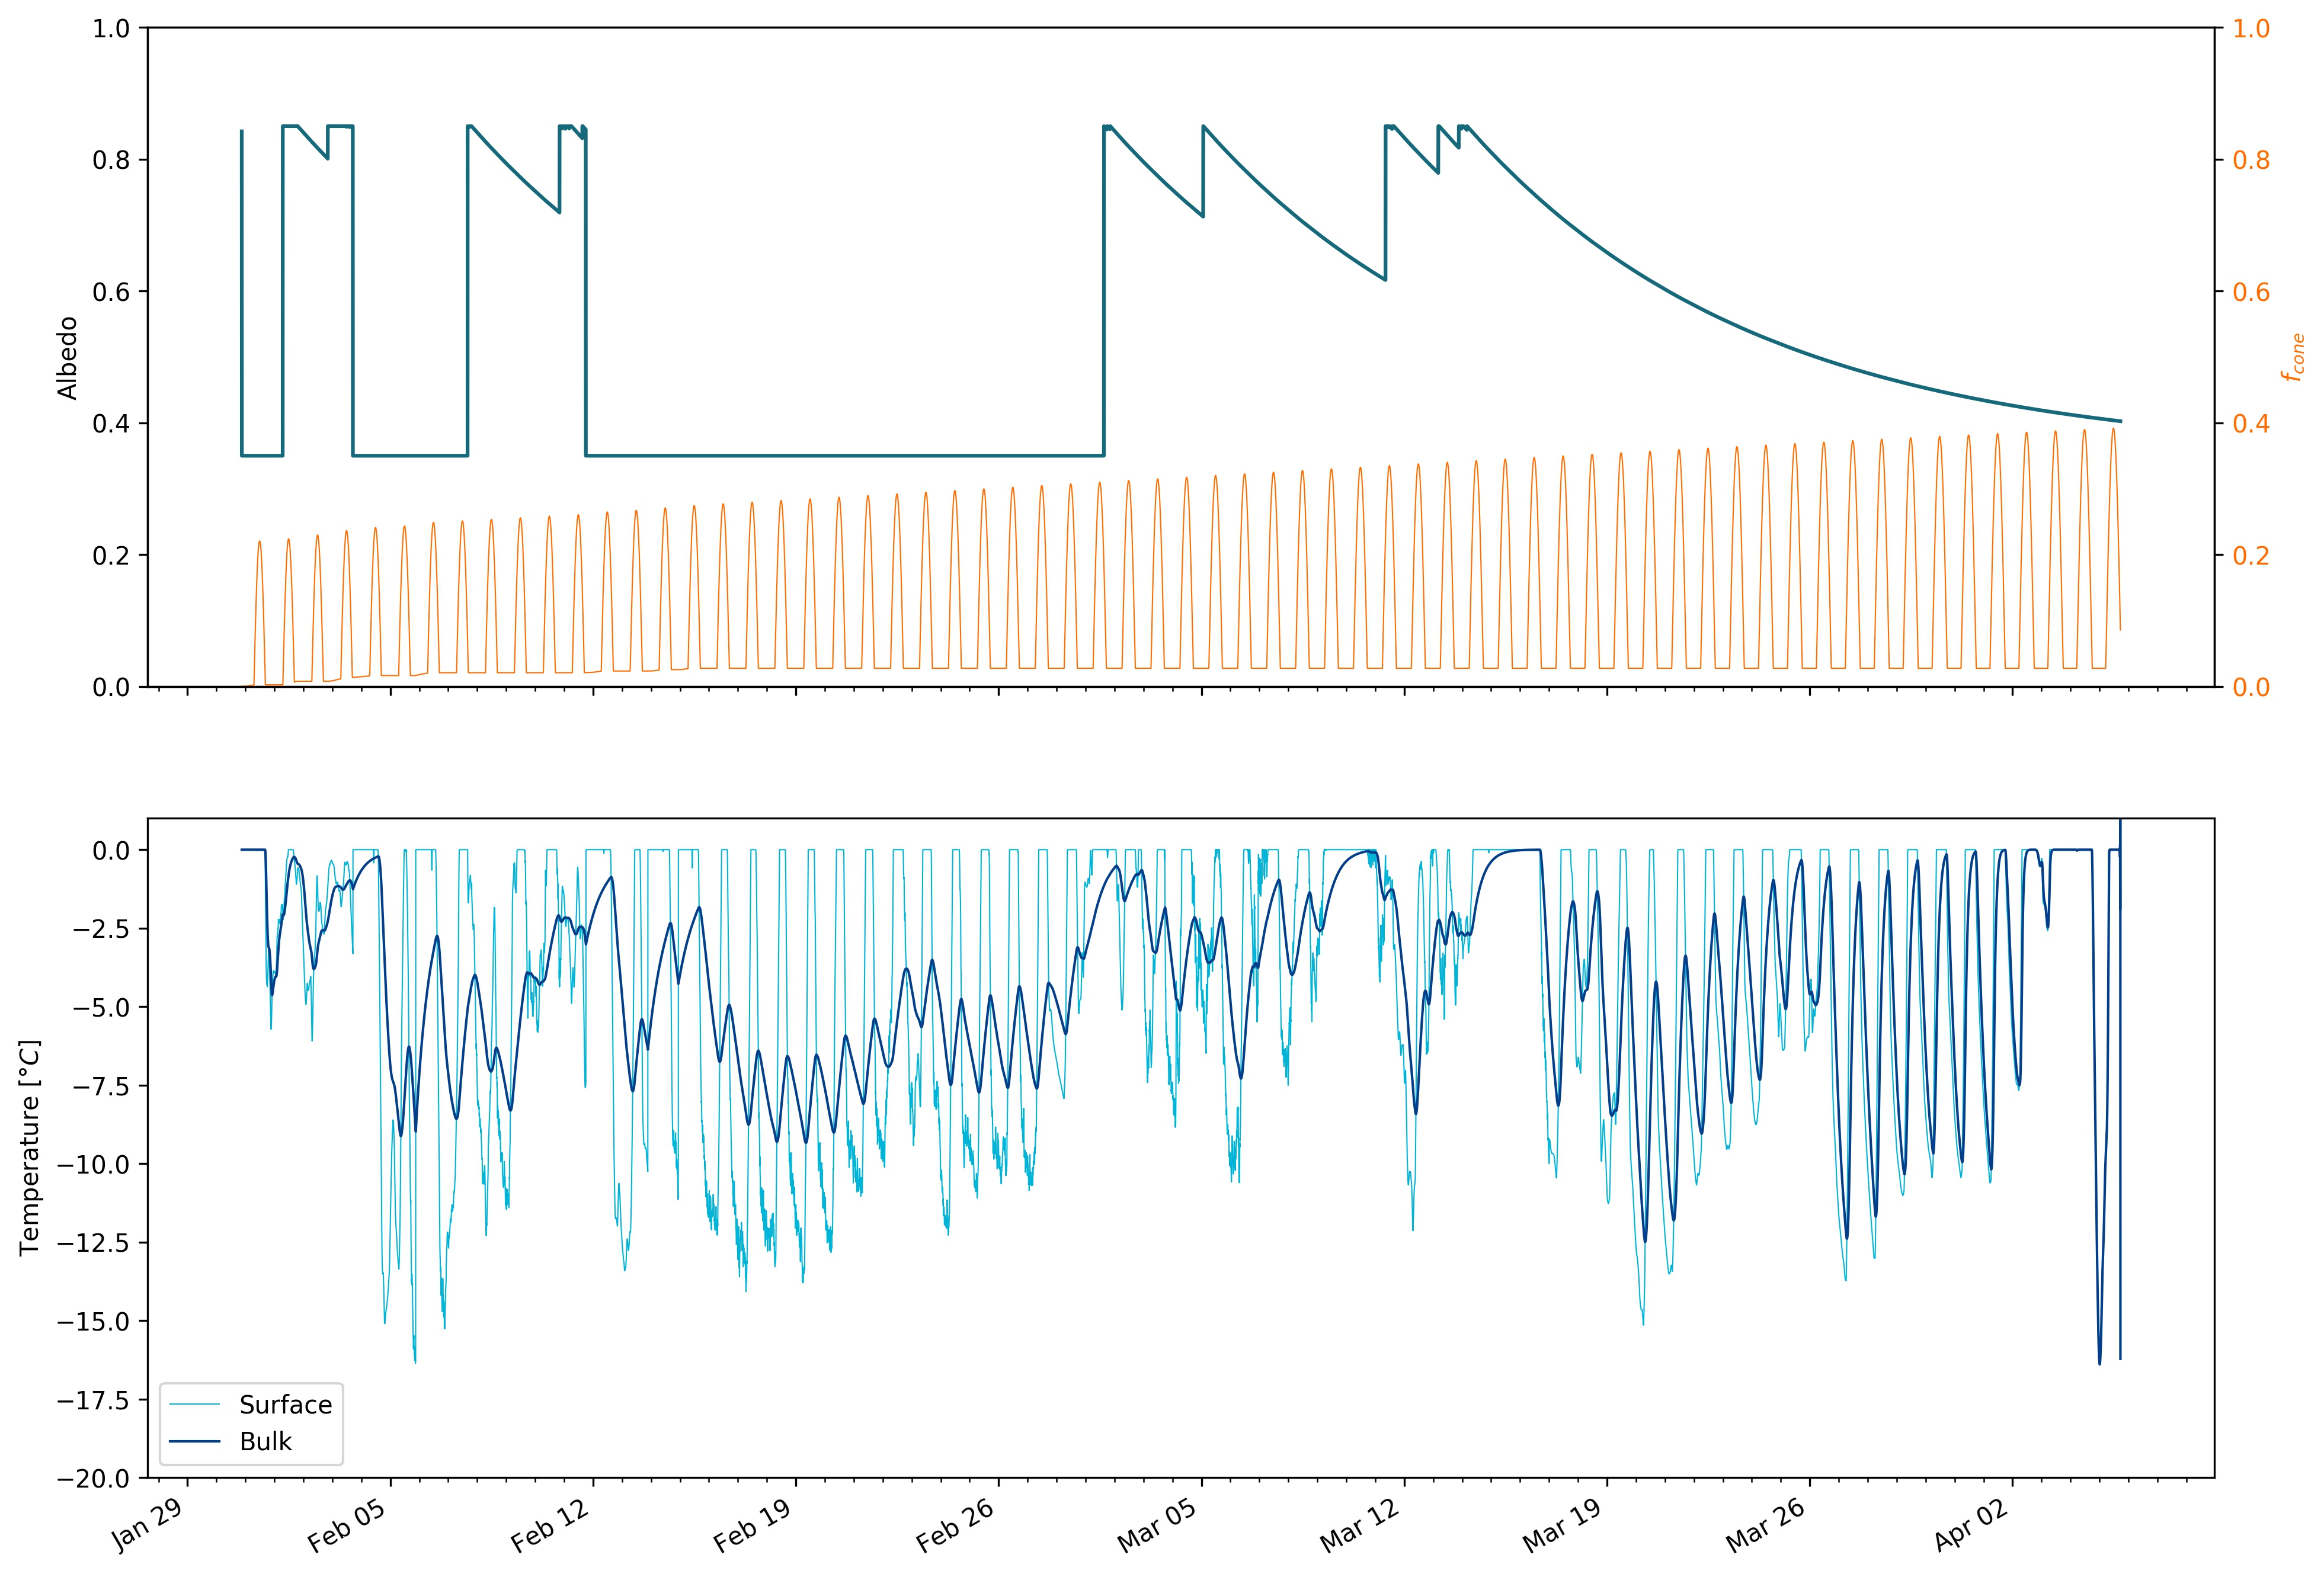
\includegraphics[width=15 cm]{Figures/Figure_7.jpg} \end{center} \caption{Some derived
  parameters of the model, namely, albedo and $f_{cone}$ (a), Surface and bulk temperature (b). In (a), the black curve
  shows how snow and fountain-on events reset albedo between ice albedo and snow albedo.  The decay of the snow albedo
  to ice albedo can also be observed. The blue curve shows how the solar radiation area fraction varied diurnally with
  variations in the solar elevation angle. In (b), the surface temperature (black curve) was forced to be 0 $\degree C$
  during fountain activity. The corresponding bulk temperature is shown with the blue curve.} \label{fig:derived}
  \end{figure}
  

\begin{table} \caption{Summary of mass balance components for the EP experiment after the fountain
  spray was stopped (on $15^{th}$ February 2019 ) and at the end of the model run (on $5^{th}$ April). All parameters
except $M_{F}$ were modelled.} \centering
    \begin{tabular}{|c|c|c|c|} \hline & \multicolumn{1}{c|}{Mass Component} & \multicolumn{1}{c|}{Fountain spray ends}
    & \multicolumn{1}{c|}{Model ends} \\
      \hline & $M_F$ & 18060 $kg$ & 18060 $kg$\\
    \parbox{2mm}{\rotatebox[origin=c]{90}{ Input }} & $M_{ppt}$ & 444 $kg$ & 467 $kg$\\
                                                    & $M_{dpt}$ & 7 $kg$ & 33
    $kg$ \\ \hline & $M_{melt}$ & 165 $kg$ & 1023 $kg$\\
    \parbox{2mm}{\rotatebox[origin=c]{90}{Output }} & $M_{ice}$ &
    814 $kg$ & 0 $kg$\\ & $M_{vapour}$ & 3 $kg$ & 8 $kg$\\ & $M_{runoff}$ & 17529 $kg$ & 17529 $kg$\\
 
 \hline \end{tabular} \label{table:MB} \end{table}


Daily averages of some components of the energy balance are shown in Fig.  \ref{fig:EB} (a). On average during the
experiment duration, the total energy flux between the atmosphere and the Icestupa are almost balanced. Net shortwave
radiation (28 $Wm^{-2}$), sensible (17 $Wm^{-2}$) and latent heat flux (9 $Wm^{-2}$) with a mostly positive flux
towards the surface of the icestupa are compensated by the net longwave radiation (- 36 $Wm^{-2}$) and the melt energy
(-19 $Wm^{-2}$). The contribution of other fluxes are negligible in comparison.

Net shortwave radiation is the main input to, and the most varying energy flux on the ice surface. Its variability is
controlled by the surface albedo $\alpha$ and the area fraction $f_{cone}$ which therefore represent key variables in
the energy balance (Fig. \ref{fig:derived} (a)). Although global radiation flux reached a daily maximum value of 304
$Wm^{-2}$, $q_{SW}$ only went up to 68 $Wm^{-2}$. This is caused by the fact that only about 30 \% of the direct
solar radiation influenced the Icestupa surface as shown by the area fraction $f_{cone}$ in Fig. \ref{fig:derived}
(a).  Snowfall is the atmospheric variable connected most closely and proportionally to albedo.  Higher and/or more
frequent snowfall thus decreases the energy available for melt due to the corresponding increase in $\alpha$. 

$q_{LW}$ was predominantly negative indicating that this energy balance component drove the freezing of the ice
structure. The incoming longwave radiation was strongly dependent on atmospheric emissivity which had a mean value of
0.77. Atmospheric emissivity in turn depended on the cloudiness factor. Daily values of $q_{LW}$ ranged from -95 to 7
$Wm^{-2}$. $q_{LW}$ and $q_{S}$ were both proportional to the temperature gradient between the air and the Icestupa
surface. Turbulent sensible heat flux $q_{S}$ contributed mostly to the melt of the ice structure. Daily values of
$q_{S}$ ranged from -16 to 59 $Wm^{-2}$. Turbulent latent heat flux $q_{L}$ was predominantly positive suggesting that
it favoured deposition/condensation over evaporation/sublimation. Daily values of $q_{L}$ ranged from -4 to 47
$Wm^{-2}$. Therefore, the Icestupa gained mass cumulatively from the atmosphere due to the deposition/condensation
process. Fountain water heat flux $q_{F}$ had a mean of zero as it was only nonzero during 1002 time steps or around
100 hours. Daily values of $q_{F}$ ranged from 0 to 7 $Wm^{-2}$. The contribution of heat flux by conduction $q_{G}$
was minimal as it only varied between -7 to 7 $Wm^{-2}$ with a mean of 0 $Wm^{-2}$. The energy contributing to surface
temperature changes ($q_{T}$) was insignificant in comparison to the energy spent on freezing and melting
($q_{melt}$).  The resulting bulk temperature and the surface temperature are shown in Fig. \ref{fig:derived} (b).
For the total considered period, $q_{LW}$ accounted for 28.3\% of overall energy turnover. The energy turnover is
calculated as the sum of energy fluxes in absolute values. $q_{SW}$ accounted for 21.7\%, followed by $q_{melt}$
(25.4\%), $q_{S}$ (14.6\%), $q_{L}$ (7.5\%), $q_{G}$ (1.8\%), $q_{F}$ (0.3\%) and $q_{T}$ (0.3\%).

Fig. \ref{fig:EB} (b) represents the mass fluxes associated with these energy exchanges expressed in $m$ w.e. It shows
the ice and meltwater formed due to $q_{melt}$, snow accumulated due to precipitation, water vapour
deposition/condensation and sublimation/evaporation due to $q_L$. Growth rate ($\frac{\Delta M_{ice}}{\Delta t}$)
shows a strong correlation with net energy flux ($r^2 = 0.44$) but poor correlation with Icestupa surface area ($r^2 =
0.04$).  This is because the variance in growth rate is mostly due to the variance in $q_{net}$ as illustrated in Fig.
\ref{fig:EB}. Since $r_{ice}$ was initialised with the spray radius $r_F$, the surface area maintains a maximum
initially until the energy flux becomes positive. This trend favours the positive over the negative thickness changes
resulting in a steep increase and gradual melting of ice volume as can be seen in Fig. \ref{fig:results}.

The total water used for the Icestupa development includes contributions from the fountain (97.2\%), snowfall (2.5 \%)
and deposition/condensation (0.3 \%) as shown in Table \ref{table:MB}. The maximum ice mass during the whole
measurement period was 1158 $kg$, which occurred after the last fountain run on Feb $16^{th}$ in the morning.
Therefore, in the case of EP we used a water input of 18,584 $kg$, with a resultant storage efficiency of only
7.5 \%.

  \begin{figure} \begin{center} 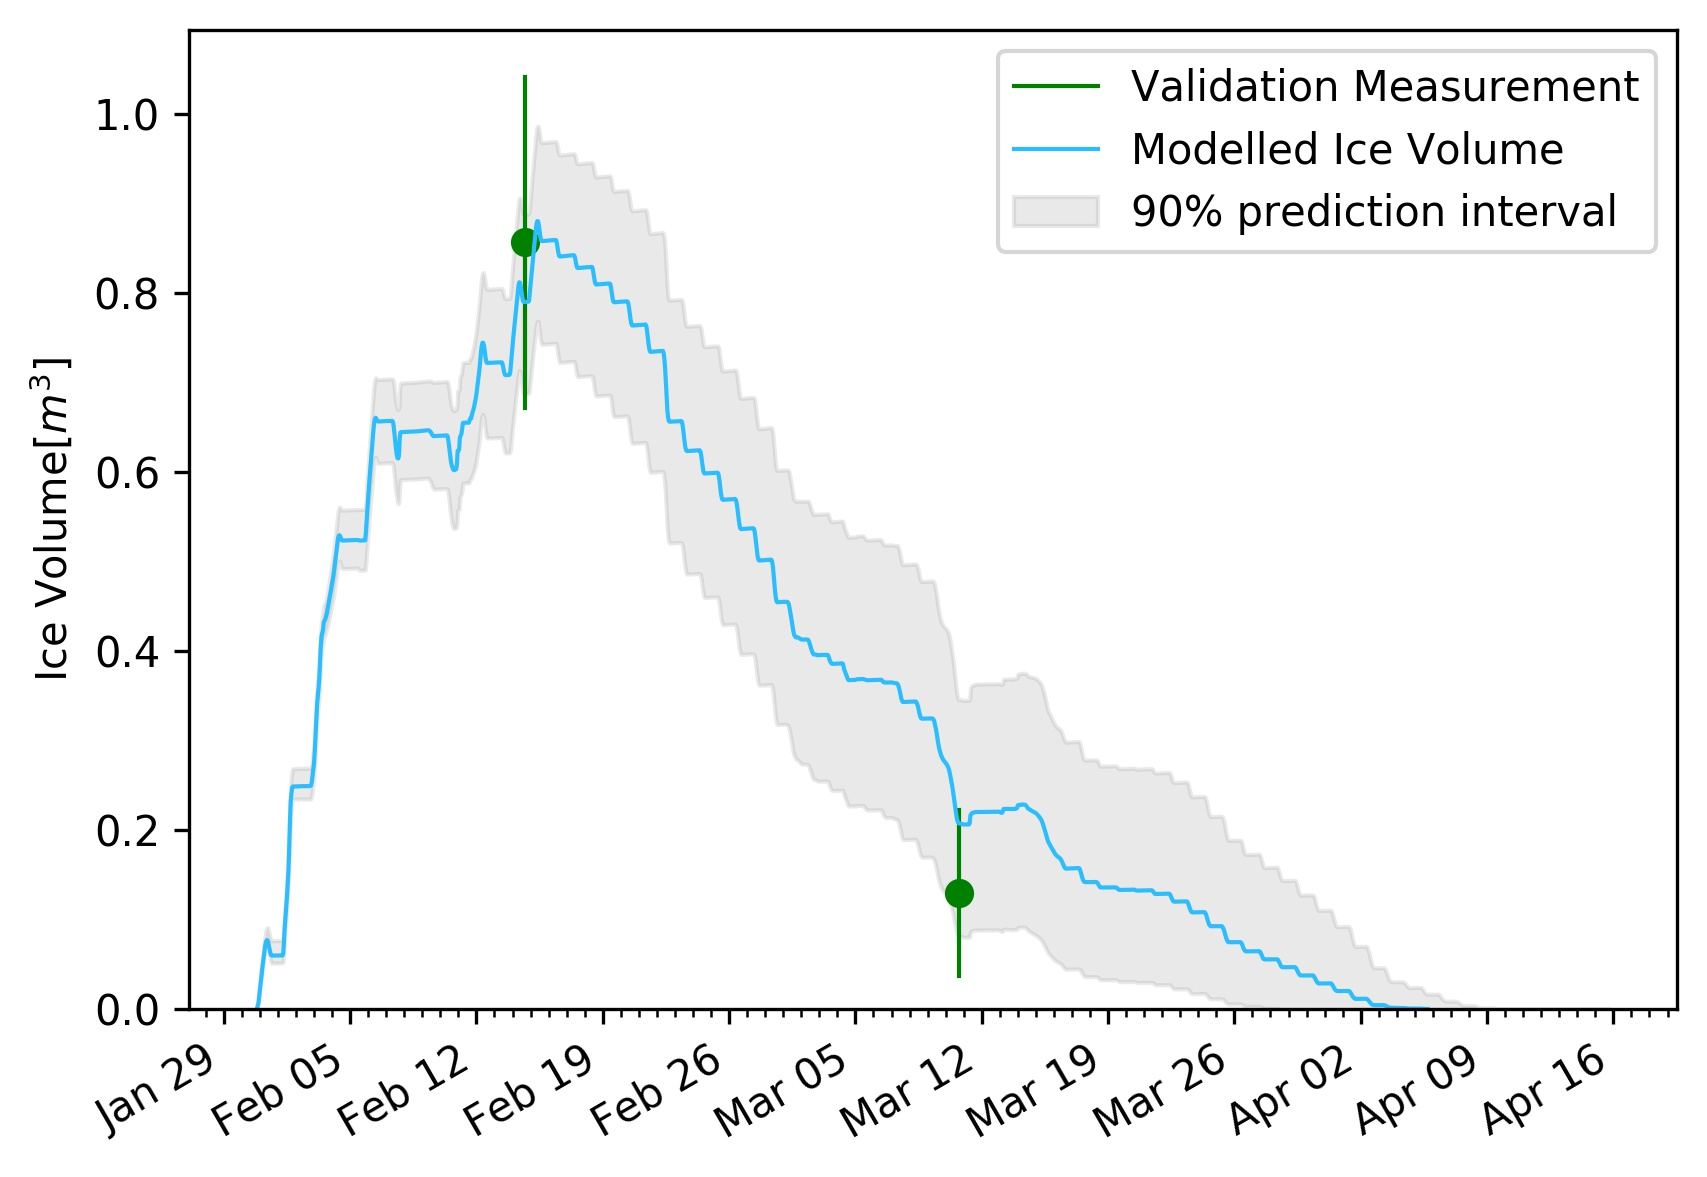
\includegraphics[width=15 cm]{Figures/Figure_8.jpg} \end{center} \caption{Modelled ice
  volume during the lifetime of the EP Icestupa (blue curve). Green line segments indicate the first and
second validation measurements. The prediction interval is based on the ice volume uncertainty caused by the most
sensitive parameters, namely, temperature threshold below which precipitation falls as snow and the ice emissivity.}
\label{fig:results} \end{figure}
  
\section{Model Sensitivity and Uncertainty analysis}

The icestupa model can be regarded as a function $f(x_1,x_2 \dots, x_n) = (y_1,y_2 \dots, y_m)$, where $(x_1,x_2
\dots, x_n)$ are the model parameters and $(y_1,y_2 \dots, y_m)$ are the model outputs. The influence of each
parameter on the output variables of interest were quantified and the most important physical parameters for the
subsequent uncertainty analysis were determined. The sensitivity of a parameter $x_j$ is determined by keeping all
other parameters $x_i, i \neq j$ fixed at their baseline value and varying $x_j$ within values that are physically
plausible.

A sensitivity study on the parameters (listed in Table \ref{table:parameters}) was performed with the maximum ice
volume as the target variable. All the parameters were assumed to be independent of each other with a uniform
distribution.  This assumption ignores the auto-correlation present among the parameters associated with the albedo
parameterisation.  The range of uncertain parameters were set based on available literature values or varied $\pm$ 5\%
from the base value if no such reference was available. The uncertainty of all the site parameters were caused due to
parallax errors during manual measurement. This was quantified with a range of $\pm$ 1\% from the base value. However,
it must be kept in mind that, even though intended to be as objective as possible, the selection of a parameter range
has a subjective part that influences the results and conclusions obtained in this analysis.  The variation of the
model outputs $y_k$ is evaluated to quantify the local sensitivities $s_{j,k}$ that are defined here as the 95\% range
of the simulated outputs.

To perform the uncertainty analysis, we included only parameters that influence the maximum ice volume by at least $0.1
m^3$. All other parameters were fixed at their baseline value.  Fig. \ref{fig:sensitivity} shows all the variance
produced by these uncertain parameters in maximum ice volume calculation. It shows that $\epsilon_{ice}$ and $T_{ppt}$
are the only parameters with a maximal sensitivity of more than 0.1 $m^3$ for the maximum ice volume estimate.
Consequently, all other parameters were excluded from the subsequent uncertainty analysis. 

The temperature threshold below which precipitation falls as snow ($T_{ppt}$) was found to be the most sensitive
parameter. It is used in the model to reset the albedo to snow albedo and determine snow precipitation events. The
lower $T_{ppt}$ parameter the higher the albedo (as the Icestupa surface has a lower albedo when ice-covered than when
snow-covered) . The variation of $T_{ppt}$ by $\pm$ $1\,\degree C$ caused maximum ice volume variation of $1.2 \pm 0.2
m^3$. 

Ice emissivity was also found to be a sensitive parameter. The higher the ice emissivity the larger the maximum ice
volume as the emitted longwave radiation increases with ice emissivity. Variation of $\epsilon_{ice}$ by 5\% caused a
maximum ice volume range from $1.3 \pm 0.1 m^3$. 

In total, the sensitivity analysis required 120 simulations, and the uncertainty analysis a total of 32 simulations.

\begin{figure} \begin{center} 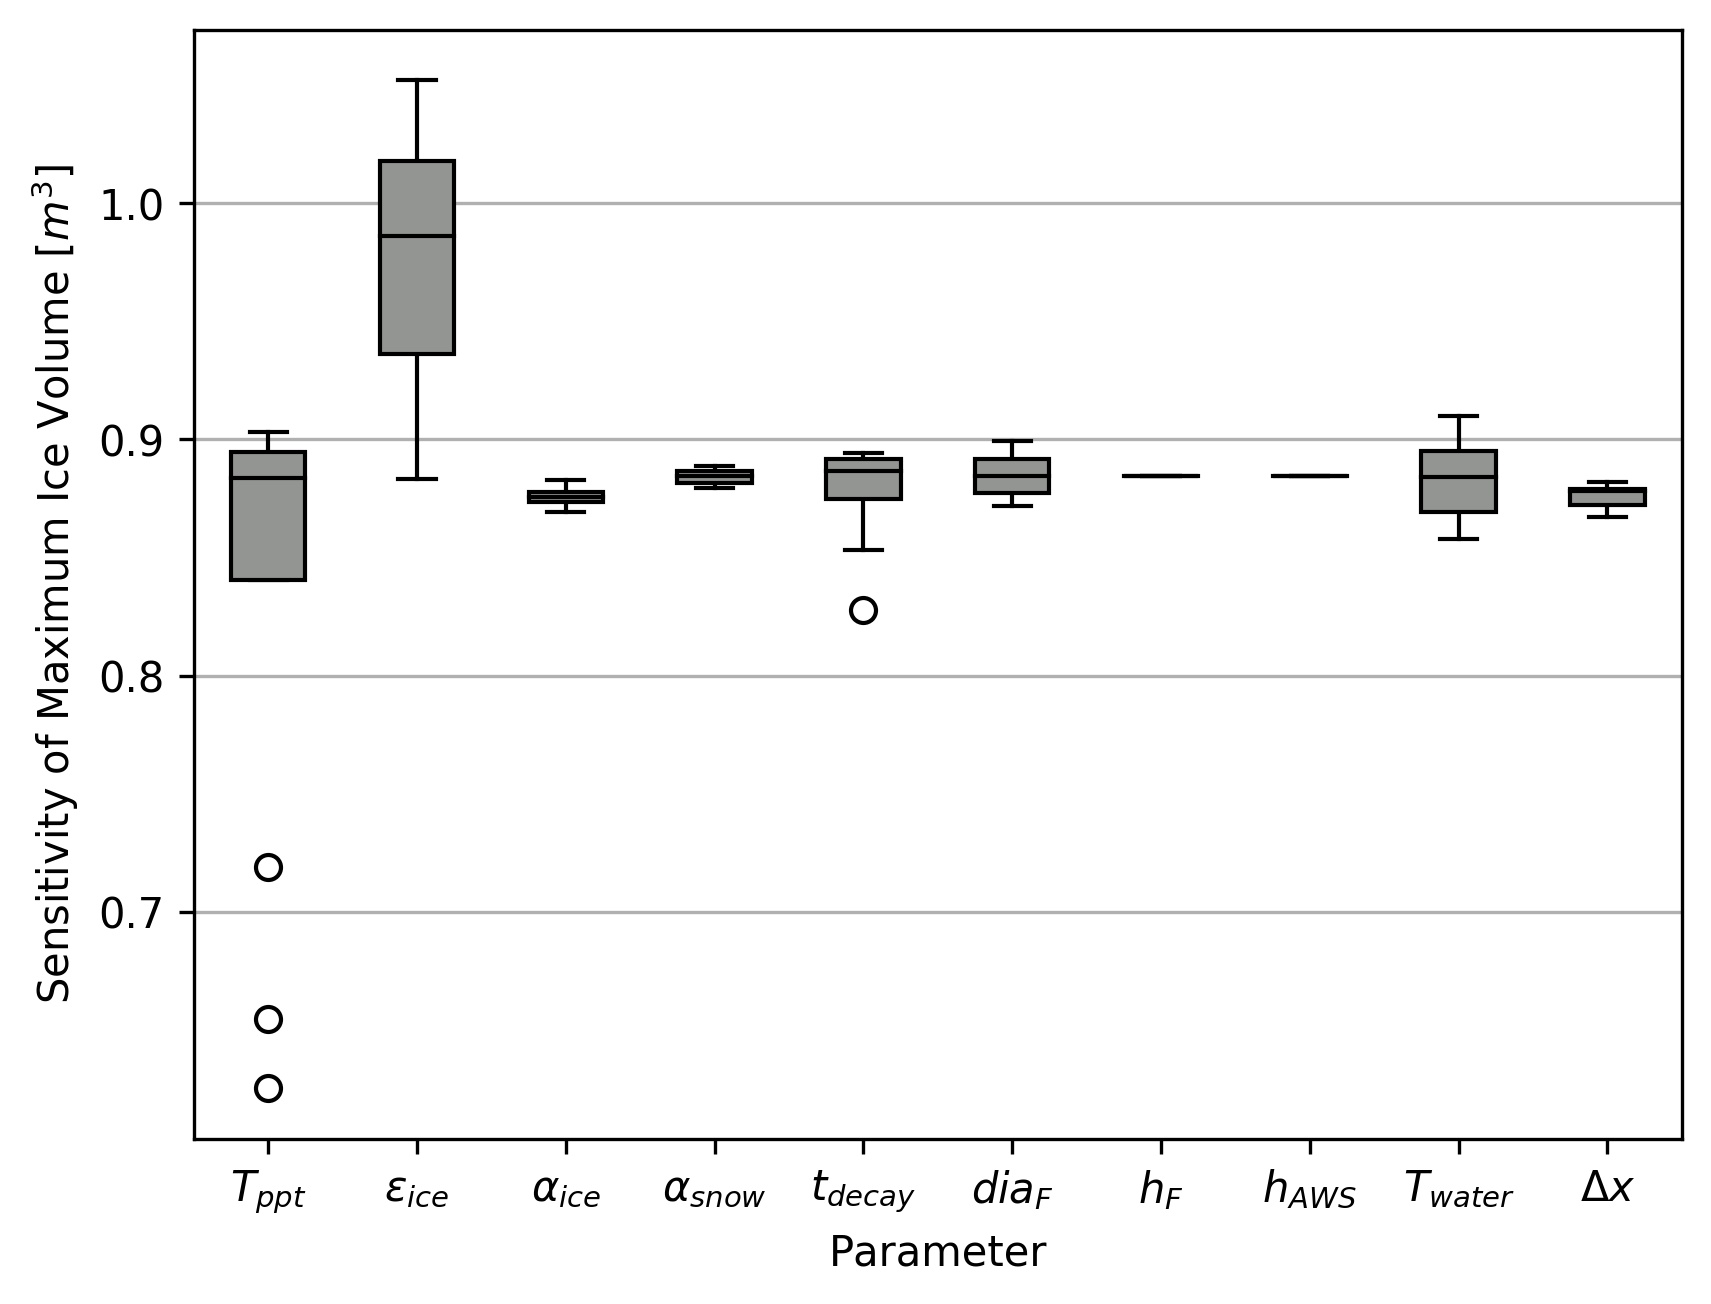
\includegraphics[width=10 cm]{Figures/Figure_9.jpg} \end{center}
\caption{Sensitivities of maximum ice volume to all the uncertain and site parameters used in the model (Table
\ref{table:parameters}).  Outliers in the bar plot are shown as 'o'.} \label{fig:sensitivity} \end{figure}
\section{Discussion}

\subsection{Model validation quality}

We first evaluate the model against the validation measurements at the EP site. The uncalibrated model is able
to capture both the freezing and the melting process sufficiently well as the modelled ice volume lies within the
uncertainty of both validation measurements. Furthermore, the validation measurements fit well within the estimated
model uncertainty.  However, since this validation is based on only two points, it does limit the confidence in the
model results. Moreover, the model seems to overestimate the ice volume at both validation points. This could be due
to the underestimation of the surface area which underestimates the melt rates (absolute growth rate when
$\frac{\Delta M_{F}}{\Delta t} < 0$) and the freeze rates(absolute growth rate when $\frac{\Delta M_{F}}{\Delta t} >
0$). However, as the fountain was mostly inactive during the study period, the underestimation of surface area
disproportionately undervalues the melt rates over the freeze rates. One major cause of this underestimation was the
conical shape assumption, as in reality, the Icestupa shape ranged between a cone and a cylinder (Fig.
\ref{fig:site}).  Another cause was the surface irregularities that were observed due to uneven exposure to direct
solar radiation and fountain droplets. The sensitivity of the model results to these errors was further amplified due
to the relatively small volume of the EP Icestupa. In summary, more validation measurements on a more
voluminous Icestupa would have increased confidence on the model results.

\subsection{Important assumptions}\label{section:assumptions} In the sensitivity and uncertainty analysis presented
above, we did not account for several general assumptions and parametrisation choices that may cause model errors.
Some assumptions and their potential to cause errors are discussed below.

\begin{itemize}

\item  Turbulent Sensible and Latent Heat Fluxes: The method used to calculate the turbulent heat fluxes by
  \cite{Garratt_1992} assumes that the turbulent heat fluxes are acting over a uniform planar surface to determine the
  roughness length. Since our application is on a conical surface, the distance to the ice surface is not
  uniform and well defined. Hence, $z_{ice}$ has no real physical significance here.

\item Droplet flight time loss: Water losses during the flight time of fountain droplets were neglected making all the
  fountain spray available for freezing. For the EP experiment, inclusion of this parameter does not influence
  results since it is already accounted for in the runoff water discharge rate which was at least $3\, l\,min^{-1}$.

\item Nucleation of droplets: Corresponding to droplet flight time, ice/snow formation is also possible before surface
  contact if nucleation occurs during flight time. For the EP experiment, this process will further increase
  the freeze rate and hence the storage efficiency. This process is neglected for model simplicity.

\end{itemize}

\subsection{Schwarzsee vs Leh Icestupa}
  
It could be argued that the relatively small EP Icestupa cannot be compared with the much larger Icestupas in
Ladakh which store millions of litres of water for several months (see Appendix \ref{section:ladakhloss}). However,
this is the only Icestupa dataset available for such a model validation.

Table \ref{table:MB} clearly shows that for our EP experiment most of the input water (92 \%) simply runoff
away. This high water loss through drainage is due to the fact that the average spray rate of the fountain
($(\frac{\Delta M_{F}}{\Delta t})_{mean} = 3.6\, l\,min^{-1}$) far exceeded the max Icestupa growth rate
($(\frac{\Delta M_{ice}}{\Delta t})_{max} = 1\, l\,min^{-1}\, \textit{(w.e.)}$ ).

In the city of Leh, Ladakh at an altitude of 3500 $m$ a.s.l. the air temperature shows values down to −27.9 $\degree
C$ in winter \citep{Chevuturi_2018} whereas EP had a minimum temperature of just -11.6 $\degree C$ during the
study period. Moreover, subzero temperatures were only reached for 7 nights of fountain operation at the EP
site compared to the 43 nights of fountain operation possible in Ladakh (see Appendix \ref{section:ladakhloss}). Thus,
the Icestupa growth rate is expected to be much higher in Ladakh. However, water spray rates in Ladakh are also much
higher (around 210 $l\,min^{-1}$). So the water losses in Ladakh could also be caused due to excessive fountain spray.

\subsection{Icestupa construction decisions} There are several decisions one has to take when constructing Icestupas.
These can be broadly divided into two types of decisions, namely fountain and location decisions.  Both the
meteorological conditions of the location and the surface area produced by the fountain significantly influence the
observed growth rate. Since our validation is restricted to just one location, we restrict our discussion to the
optimization possibilities of Icestupa constructions through fountain decisions.

  \begin{figure} \begin{center} 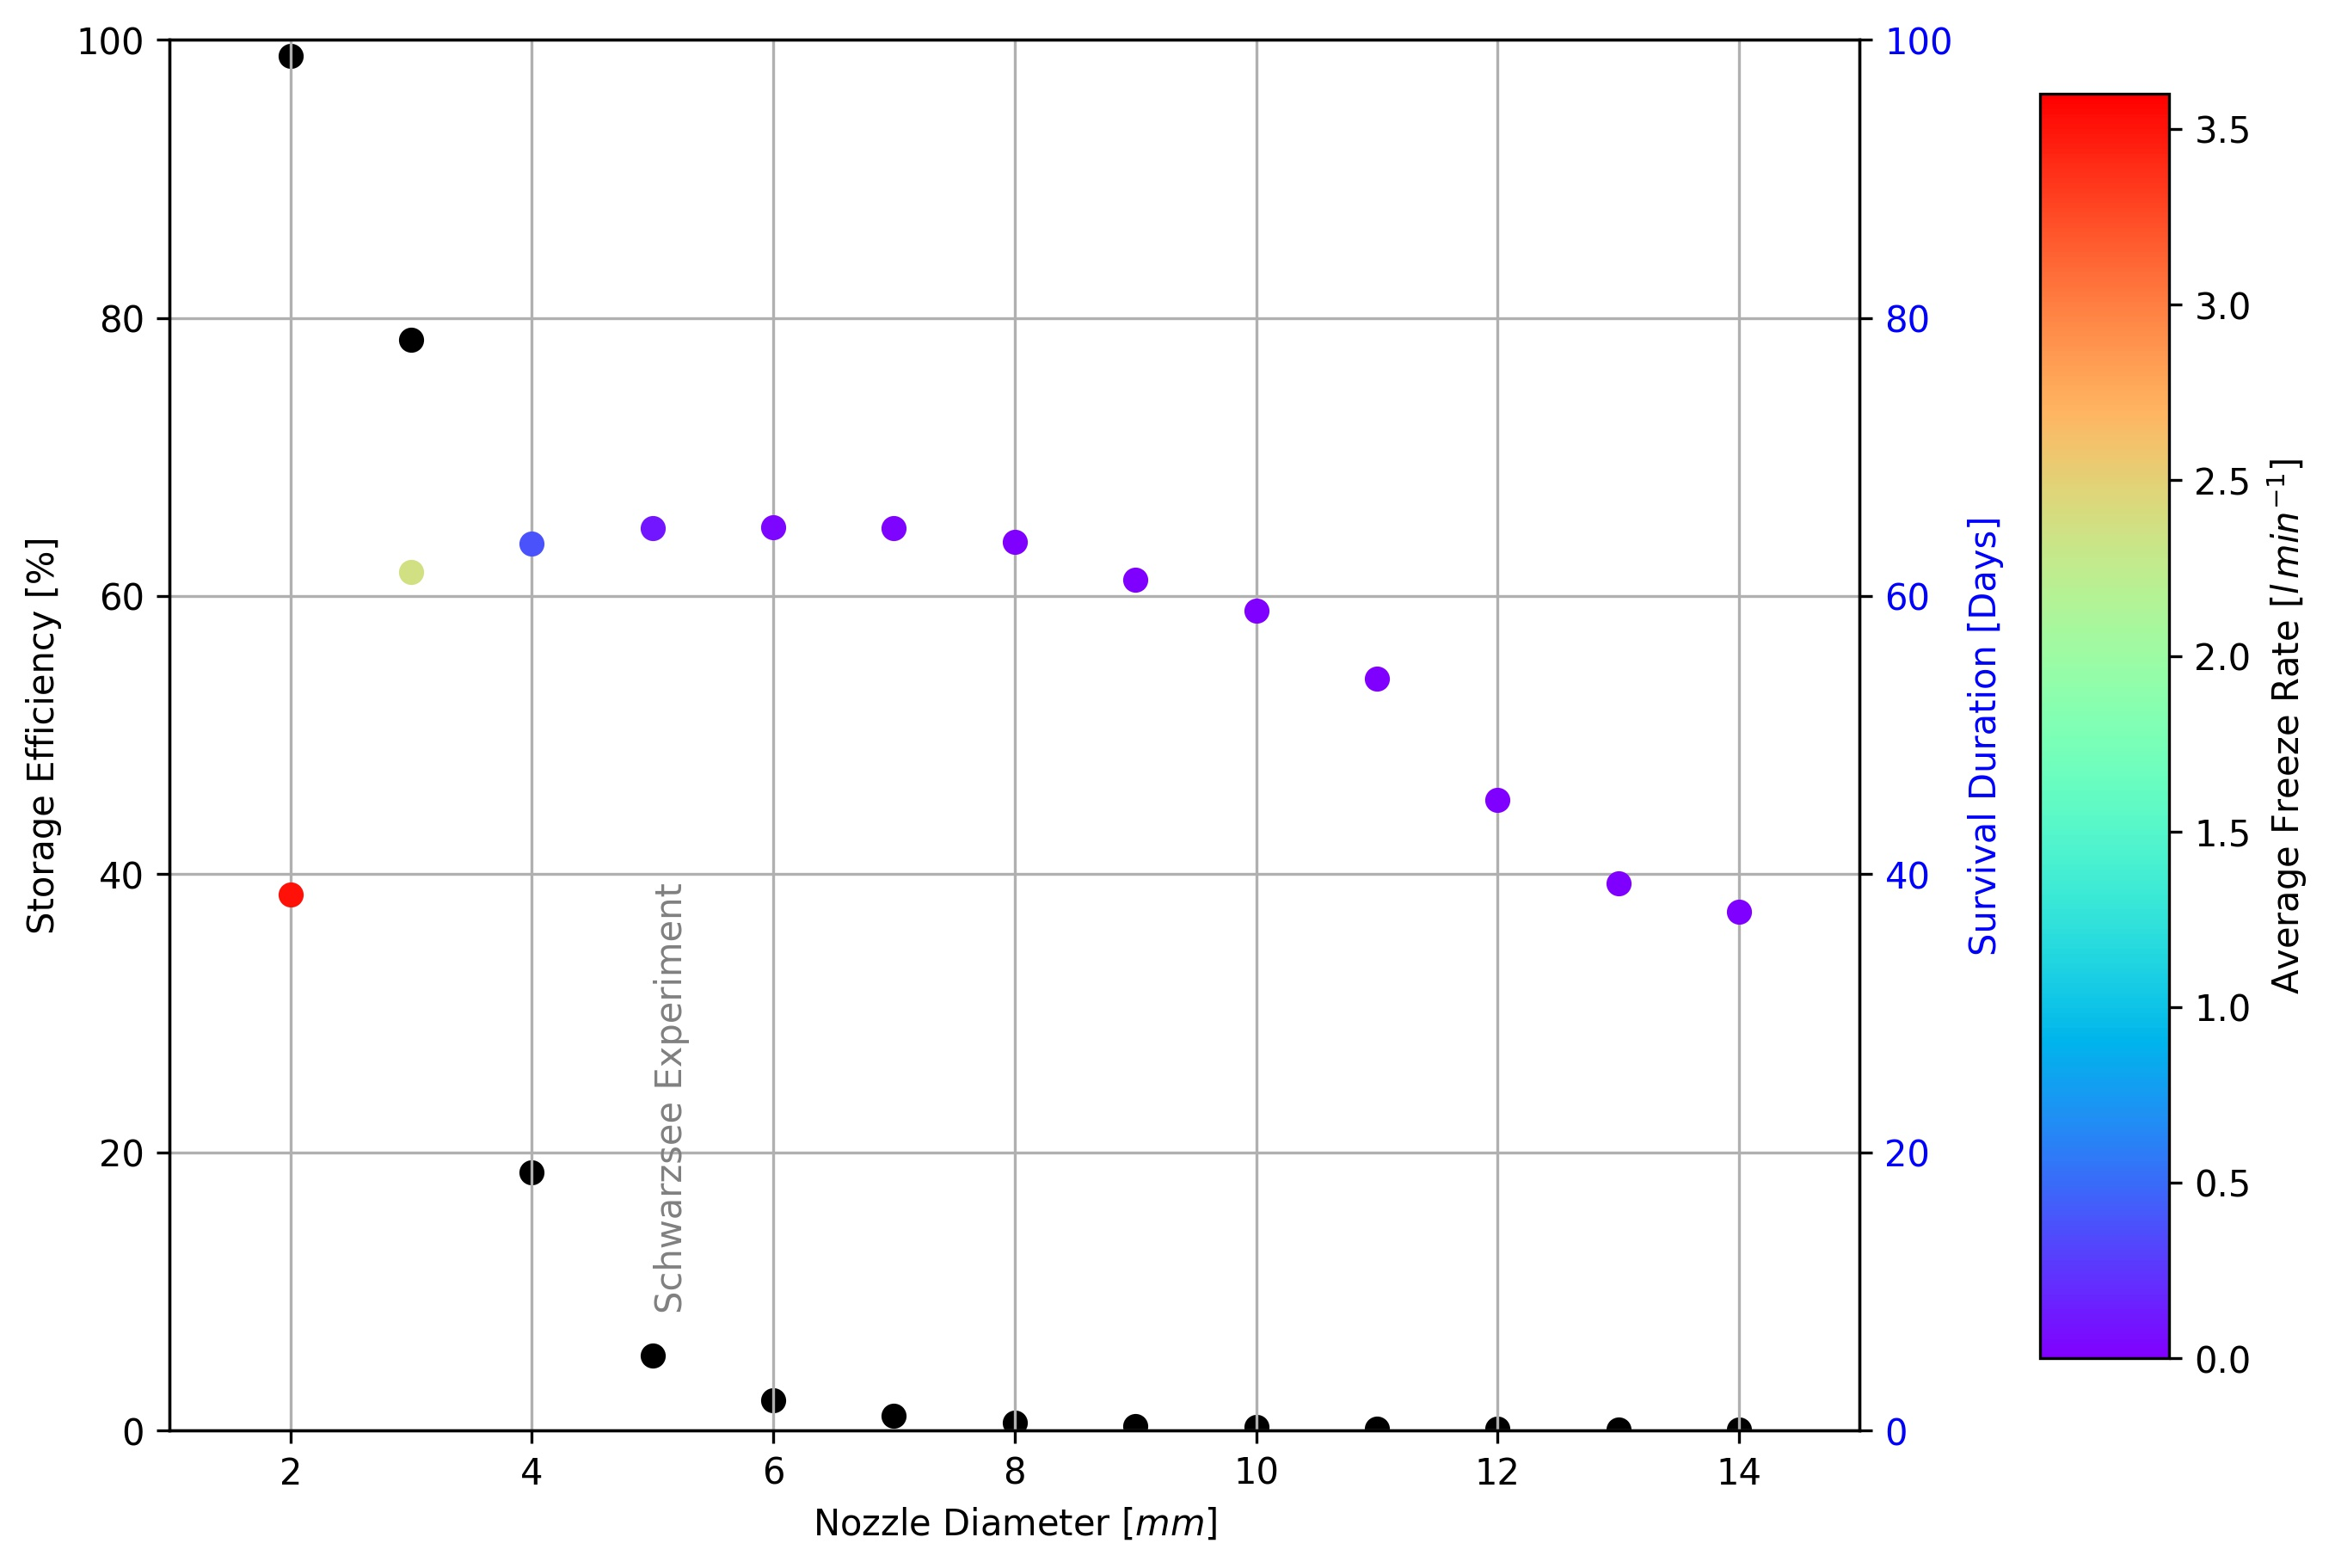
\includegraphics[width=15 cm]{Figures/Figure_10.jpg} \end{center} \caption{Variation
in storage efficiency (black dots) and storage duration (coloured dots) with changes in fountain nozzle's nozzle
diameter.  The dot colours represent average freeze rate based on the color bar.} \label{fig:dia_f} \end{figure}
  

Assuming a constant spray for the fountain, we can divide the fountain decisions into fountain state (on/off) and type
(height and nozzle diameter).  From an energy balance point of view, the fountain should be switched on for all time
intervals when $q_{net} < 0$. However, in our experiment, the fountain state decision was set based on whether the
ambient temperature was above or below a critical temperature of $-5 \degree C$. Ambient temperature can serve as an
indicator of $q_{net}$ as it was correlated ($r^2 = 0.53$).  However, $q_{net}$ was found to be negative already at a
critical temperature of $-1 \degree C$. Therefore, using air temperature to determine when the fountain should be
switched on is justified but a higher critical temperature could have been used in the case of the EP
Icestupa. 

The fountain type used can be characterised by the physical structure of the fountain, namely its height and nozzle
diameter. Maintaining the same spray rate and height, one can optimize the Icestupa development by identifying the
minimum nozzle diameter that yields the maximum storage efficiency. 

Fig. \ref{fig:dia_f} shows reducing the nozzle diameter to 3 $mm$ increases storage efficiency up to 93 \% without
compromising much on storage duration.  The corresponding storage quantity of the 3 $mm$ nozzle diameter was more than
20 times higher than the 5 $mm$ fountain used in our experiment. This is because the spray radius $r_F$ of the 3 $mm$
fountain was much higher at 8.5 $m$ compared to the 1.7 $m$ spray radius of the 5 $mm$ fountain (see Appendix Section
\ref{section:rF}). Here, we define growth rate as freeze rate when fountain is active and melt rate otherwise. So this
higher spray radius both, increases the freeze rate  and increases the melt rate since they are both directly
proportional to the surface area. However, since the freeze rate cannot increase beyond a spray rate of 3.6 $l
min^{-1}$ (except during precipitation or deposition/condensation events), an optimum spray radius or nozzle diameter
exists, beyond which storage duration suffers due to a disproportionate increase in melt rate compared to the freeze
rate. So even though 3 $mm$ nozzle diameter had a much higher storage quantity than the 5 $mm$ nozzle, its storage
duration was around 6 days less than the 5 $mm$ nozzle. One physical cause of this effect is the different shapes of
both the ice structures. A flat sheet of ice (effectively a cone with a high spray radius) with higher mass might have
a storage duration shorter than a conical ice structure. As the spray radius decreases with increasing nozzle
diameter, the ice structure’s average slope increases and so the 5 $mm$ nozzle's ice structure is "more" conical than
the 3 $mm$ ice structure. Fig.  \ref{fig:dia_f} shows that a nozzle diameter of 3 $mm$ has an average freeze rate (3.2
$l \,min^{-1} w.e.$) which is large enough to increase the storage efficiency and small enough to not reduce the
storage duration of the Icestupa significantly.

\subsection{Artificial snow production vs Artificial ice reservoirs}
Both Artificial snow and ice are produced by expelling small liquid water droplets from the snow gun or fountain
nozzles at high speed \citep{BoundaryConditionsforArtificialSnowProductionintheAustrianAlps}. The crucial factor that
determines ice or snow production is whether these water droplets remain unfrozen or freeze before reaching the
ice/snow surface. According to \citep{HARTL2018123}, the production potential of artificial snowmaking is proportional
to the wet-bulb temperature and the threshold mean daily wet bulb temperature for potential snow making days was $- 2
\, \degree C$ which corresponds well with the threshold mean daily air temperature for potential ice making days of EP
site ($- 1 \, \degree C$).

\section{Conclusions} We outlined a methodology for estimating ice, liquid water, water vapour and runoff
quantities produced during the construction of an Icestupa using m:easurements of fountain spray rate, air temperature,
radiation, humidity, pressure, wind and cloudiness at the EP study site. The comparison with validation
measurements at two different dates during the experiment led to satisfying results, although a more rigorous model
validation was not possible due to few icestupa volume measurements.

According to the model, the EP Icestupa achieved a storage quantity of 1392 litres of water with a storage
duration of 61 days. However, the corresponding storage efficiency was very low with only 7.5 \% for a water input of
18,584 litres. These estimates were most sensitive to the temperature threshold that determined precipitation phase
and ice emissivity parameters which created an uncertainty of $1.2 \pm 0.3 m^3$ in the maximum ice volume calculated.
This is to be expected as net longwave radiation and net shortwave radiation together accounted for around 50 \% of
the overall energy turnover.

Although the location, storage quantity and duration of our experimental EP Icestupa are not representative of
the much larger Icestupas of Ladakh, the model results do support the hypothesis that there could be considerable
water loss during the formation of Icestupas particularly due to excessive fountain spray. Using model calculations,
it was shown that a decreased fountain nozzle diameter of 3 $mm$ can increase the storage efficiency drastically. This
is because a change in the fountain nozzle diameter causes an effective change of the ice surface area over which the
net energy flux can act. This result has relevance on the future design of Icestupa fountains. However, care has to be
taken as our model is currently only validated by one experiment at the EP site. Further experiments at
different locations with different fountains are required to better understand the influence of construction decisions
on the results. 



\section{Appendix}

\subsection{Ladakh Icestupa 2014/15} \label{section:ladakhloss} A 20 $m$ tall Icestupa \citep{iceheight} was built in
Phyang village, Ladakh at an altitude of 3500 $m$ a.s.l. Assuming a conical shape with a diameter of 20 $m$, the
corresponding volume of this Icestupa becomes 2093 $m^3$ or 1,919,587 litres w.e. The fountain sprayed water at a rate
of $210\, l\,min^{-1}$ \citep{waterinput} from $21^{st}$ January \citep{waterstart} to at least until $5^{th}$ March
2015 \citep{waterend} (around 43 nights). Assuming fountain spray was active for 8 hours each night, we estimate water
consumption to be around 4,334,400 litres. So just during construction/freezing period of the Icestupa, roughly 56 \%
of the water provided was wasted. The actual water loss is bound to be much higher due to further vapour losses during
the melting period. This Icestupa completely melted away on $6^{th}$ July 2015 \citep{iceends}. Therefore, the storage
duration was 166 days or roughly 5 months. 


\section*{Conflict of Interest Statement} The authors declare that the research was conducted in the absence of any
commercial or financial relationships that could be construed as a potential conflict of interest.

\section*{Author Contributions} SB wrote the initial version of the manuscript. MH, ML, SW, JO, and FK commented on
the initial manuscript and helped improve it. SB developed the methodology with inputs from MH. SB performed the
analysis with support from MH and ML. SB and MH participated in the fieldwork.

\section*{Funding} This work was supported and funded by the University of Fribourg and by the Swiss Government
Excellence Scholarship (Suryanarayanan Balasubramanian).

\section*{Acknowledgments} We thank Mr. Adolf Kaeser and Mr. Flavio Catillaz at Eispalast Schwarzsee for their active
participation in the fieldwork. We would also like to thank Digmesa AG for subsidising their flowmeter used in the
experiment. We would particularly like to thank the editor Prof. Thomas Schuler who gave us important inputs to
improve the paper and we thank also Prof. Christian Hauck and Prof. Nanna B. Karlsson for valuable suggestions that
improved the manuscript.


\section*{Data Availability Statement} The data and code used to produce results and figures will be published at a
later stage and can, until then, be obtained from the authors upon request.

\bibliographystyle{frontiersinSCNS_ENG_HUMS} \bibliography{references}

\end{document}
